\documentclass[11pt,a4paper]{article}

% Provisional/scratch companion to paper.tex. Holds figures and tables that
% may belong in the final thesis but are currently not load-bearing for the
% headline (within-day DiD on q_2). Each block is captioned with its
% provisional status so the reader knows it's exploratory.

\PassOptionsToPackage{table}{xcolor}
\usepackage{amsmath, amssymb, amsthm, mathtools}
\usepackage{graphicx, booktabs, subcaption, tikz, float}
\graphicspath{{../../figures/thesis/}}
\usepackage{array, makecell, multirow}
\usepackage{xcolor}
\usepackage{longtable}
\usepackage[hidelinks]{hyperref}
\usepackage{geometry}
\geometry{a4paper, margin=2.5cm}
\usepackage{caption}
\captionsetup{font=small, labelfont=bf}

% \code{...} -- monospace code/path that allows line breaks at _ and /.
% Uses url package's hyphenation hooks; reads underscores literally (no \_ needed).
\usepackage{url}
\urlstyle{tt}
\Urlmuskip=0mu plus 1mu\relax  % allow stretchy break-points so long paths wrap
\def\UrlBreaks{\do\/\do\_\do\-\do\.\do\:\do\,}
\newcommand{\code}[1]{\nolinkurl{#1}}

\title{Provisional figures and tables\\[3pt]\large MTU15 thesis (companion to paper.tex)}
\author{Pablo Paramio}
\date{\today}

\begin{document}
\maketitle

\noindent\emph{This file is exploratory scratch space. None of these objects is currently cited from \texttt{paper.tex}. They are kept here for inspection and decision-making — promote to the main paper if the empirical content is load-bearing, otherwise leave here or move to \code{attic/}.}

\tableofcontents


% =====================================================================
\section{Reform-window identification (DA15 + IDA15)}\label{sec:prov:reform_window_ddd}
% =====================================================================

\noindent The headline thesis question is the effect of \textbf{MTU15 granularity} on strategic bidding. Reforzada (the post-blackout RT2 pay-as-bid + zonal-monopoly windfall channel documented in \S\ref{sec:prov:phf_minus_pdbf}--\S\ref{sec:prov:geo}--\S\ref{sec:prov:cournot_cnmc}) is a parallel \emph{confounding} mechanism --- analogous in spirit to the operational/solar midday channel in the main paper (\texttt{paper.tex}~§2.4): a real economic phenomenon that we want to characterise but \emph{exclude from the identifying contrast} so as not to mix channels. This section's design picks reform windows in which reforzada is held constant, then differences out residual seasonality via a 2024 placebo.

\paragraph{Design.} Two reform-windows, each chosen so that reforzada is constant within both the pre- and post-treatment sub-windows:

\begin{table}[H]
\centering
\caption{Reform-window design. Reforzada is the post-blackout RT2 pay-as-bid regime (active 2025-04-28 onward). The 2024 placebo uses calendar-matched dates. PT assumption: YoY seasonal change in (crit $-$ flat) was the same in 2024 as in 2025.}
\label{tab:reform_windows}
\footnotesize
\setlength{\tabcolsep}{4pt}
\begin{tabular}{@{}l l l c c@{}}
\toprule
Reform / sample & Pre-window & Post-window & Reforzada & Length pre/post \\
\midrule
\textbf{IDA15 (2025)} & 2024-12-09 -- 2025-03-18 & 2025-03-19 -- 2025-04-27 & off & 100 / 40 d \\
IDA15 placebo (2024)  & 2023-12-09 -- 2024-03-18 & 2024-03-19 -- 2024-04-27 & off & matching \\
\addlinespace
\textbf{DA15 (2025)} & 2025-04-28 -- 2025-09-30 & 2025-10-01 -- 2026-02-13 & on  & 155 / 135 d \\
DA15 placebo (2024)  & 2024-04-28 -- 2024-09-30 & 2024-10-01 -- 2025-02-13 & off & matching \\
\bottomrule
\end{tabular}
\end{table}

\textit{Reading} (\textbf{supportive, by design}). DA15 holds reforzada constant (on) in both sub-windows; IDA15 holds it constant (off). Each pre-window is $\ge 3$ months; DA15 has 5 months post-reform.

\textit{Verdict} (\textbf{supportive}). Temporal design isolates each MTU15 reform from reforzada. The 2024 placebo provides the seasonality control absent on the within-day DiD alone.

\begin{figure}[H]
\centering
\includegraphics[width=0.95\textwidth]{../../figures/working/fig_reform_windows_timeline.pdf}
\caption{\textbf{Timeline of reforms and DDD windows.} Vertical guides: ISP15 (2024-12-09), MTU15-IDA (2025-03-19), Iberian blackout (2025-04-28), MTU15-DA (2025-10-01). Shaded grey: reforzada zone. Blue bars: pre-reform sub-windows; red bars: post-reform. 2024 placebo rows shown with lighter shading.}
\end{figure}

\textit{Reading} (\textbf{supportive}). Visual confirmation: DA15 windows sit entirely inside the reforzada zone; IDA15 windows entirely outside.

\paragraph{Triple-difference specification.}
Let $Y_{f,u,d,h}$ be the outcome at firm $f$, unit $u$, date $d$, clock-hour $h$. Define $\text{crit}_h = 1$ if $h \in \{5\!-\!9,\,16\!-\!22\}$ (treated hour-class), restrict sample to $\{\text{crit}, \text{flat}\}$. Let $\text{post}_d = 1$ if $d$ is after the reform date, $\text{y25}_d = 1$ if $d$ falls in the 2025 (treatment) window. Then:
\begin{multline}
  Y_{f,u,d,h} = \alpha + \beta_1 \text{crit}_h + \beta_2 \text{post}_d + \beta_3 \text{y25}_d
    + \beta_4 (\text{crit} \times \text{post}) + \beta_5 (\text{crit} \times \text{y25}) \\
    + \beta_6 (\text{post} \times \text{y25})
    + \boxed{\beta_7 (\text{crit} \times \text{post} \times \text{y25})}
    + \gamma_f + \mu_u + \delta_{\text{DOW}(d)} + \varepsilon_{f,u,d,h}.
\end{multline}
$\beta_7$ is the headline coefficient: the change in the (critical $-$ flat) differential at the reform date, \emph{net of} the corresponding 2024 seasonal change. FE: firm $\gamma_f$ + unit $\mu_u$ + day-of-week $\delta_{\text{DOW}}$. SE clustered at the date level. Equivalently $\beta_7 = \Delta\Delta Y^{2025} - \Delta\Delta Y^{2024}$ where $\Delta\Delta Y = (\bar Y_{\text{post,crit}} - \bar Y_{\text{post,flat}}) - (\bar Y_{\text{pre,crit}} - \bar Y_{\text{pre,flat}})$.

\paragraph{Event-study spec (visual pre-trends).} For each outcome, plot the monthly differential separately for the 2025 treatment year and the 2024 placebo year, anchored to $\tau =$ months from the reform date:
\[
  \Delta Y_{\tau,y} \;=\; \bar Y_{\text{crit}}(\tau, y) - \bar Y_{\text{flat}}(\tau, y), \qquad y \in \{2024, 2025\}.
\]
Identifying assumption test: for $\tau < 0$ the two series should overlap (parallel pre-trends); at $\tau \ge 0$ the 2025 series diverges from the 2024 series by exactly the treatment effect.

\paragraph{Identifying assumptions.}
\textit{Formal PT (triple-difference).}
\[
  \mathbb{E}\big[\Delta\Delta Y(0) \mid \text{y25}=1\big] \;=\; \mathbb{E}\big[\Delta\Delta Y(0) \mid \text{y25}=0\big],
\]
where $\Delta\Delta Y(0)$ is the untreated within-day pre/post change in the critical-flat differential.

\textit{Threats killed by the design.}
\begin{itemize}
   \item \emph{Seasonality of the critical-flat spread} (summer-to-winter heating/AC patterns): differenced out by the 2024 placebo on the same calendar months.
   \item \emph{Day-level cost shocks} (TTF gas, CO$_2$, demand spikes): within-day differencing on each date absorbs anything that hits both hour-classes proportionally.
   \item \emph{Asymmetric gas-cost confound}: ruled out empirically in \texttt{paper.tex}~§2.4 --- CCGT price-setting share 9.1\% crit vs 9.0\% flat, so TTF shocks cannot propagate asymmetrically.
   \item \emph{Operational midday channel} (solar drives prices down at midday): midday hours $\in \{11\!-\!14\}$ excluded from the control set; only flat hours $\in \{1,2,3\}$ enter as control.
   \item \emph{Reforzada / RT2 pay-as-bid windfall}: held constant within each window by design (the central insight). Characterised as confounder in \S\ref{sec:prov:phf_minus_pdbf}--\S\ref{sec:prov:geo}--\S\ref{sec:prov:cournot_cnmc}.
\end{itemize}

\textit{Threats remaining.}
\begin{itemize}
   \item \emph{Within-firm portfolio composition shifts}: addressed by unit FE; sensitivity check restricts to units active in both years.
   \item \emph{Reform-anticipation effects}: tested by the event-study leads $\beta_\tau$ for $\tau \in \{-1, -2\}$.
\end{itemize}

\paragraph{Extension to $k$-way DiD (pivotal moderator).} The main paper's appendix already runs a triple-difference with $\text{pivotal}_f \in \{0, 1\}$ (Big-4 dominant firms vs non-pivotal placebos). Adding the 2024 placebo as a fourth axis gives a \textbf{quadruple difference}. The estimable spec, after dropping the $\text{pivotal}_f$ main effect (firm-invariant, absorbed by $\gamma_f$):
\begin{multline}
  Y_{f,u,d,h} = \alpha + \beta_1 \text{crit} + \beta_2 \text{post} + \beta_3 \text{y25}
    + \sum_{\text{6 pairs involving } \text{crit, post, y25, pivotal}} \\
    + \sum_{\text{4 triples involving time-varying axes}}
    + \boxed{\beta_{1234}\,(\text{crit} \times \text{post} \times \text{y25} \times \text{pivotal})}
    + \gamma_f + \mu_u + \delta_{\text{DOW}(d)} + \varepsilon.
\end{multline}
The pivotal main effect and any pivotal $\times$ (firm-invariant) interaction are dropped — absorbed by firm FE $\gamma_f$. All 6 pairs and all 4 triples that involve at least one within-firm-varying axis (crit, post, y25) are kept.

\textit{Sample restriction for the DDDD}. To avoid contamination from the June 2024 IDA reform (6$\to$3 sessions) and the December 2024 ISP15 rollout, the DDDD sample is restricted to \textbf{Jan--May 2024 (placebo) vs Jan--May 2025 (treatment)}. The 2-month post-IDA15 window (Mar 19 -- Apr 27 2025) sits inside this restriction; the 2024 placebo correspondingly uses Mar 19 -- Apr 27 2024.

\textit{SE clustering}. Cluster at the \textbf{firm} level, not the unit level: pivotal does not vary within firm, so within-firm error correlation is the relevant dependence.

\textit{Interpretation}. $\beta_{1234}$ identifies the \emph{pivotal-differential} MTU15 effect on the critical-flat differential --- whether pivotal firms respond more strongly than non-pivotal firms, net of all lower-order interactions. It is a direct test of the \emph{market-power mechanism}: a significant $\beta_{1234} > 0$ (in the strategic-exploitation direction) or $< 0$ (operational direction) would indicate the effect is concentrated in the firms with pivotality. \textbf{Non-rejection of $\beta_{1234} = 0$ does \emph{not} rule out a uniform-effect mechanism} in which all firms respond similarly to the reform --- which would still show up in $\beta_7$. The two coefficients answer different questions: $\beta_7$ is the average reform effect; $\beta_{1234}$ is the pivotal-incremental effect. We will report both with their CIs side-by-side so the power gap (the DDDD necessarily has wider SE because it conditions on a higher-order interaction) is visible.

\paragraph{Outcomes.} Three outcomes, each with its own identifying assumption and economic story. $D_w / \Delta p / \Delta q$ are \emph{not} DDD outcomes --- they require within-hour quarters that do not exist pre-MTU15 (see \S\ref{sec:prov:dw_decomp}, \S\ref{sec:prov:dw_distributions} for the post-only cross-section).

\begin{table}[H]
\centering
\caption{DDD outcomes, with competing theoretical predictions. The headline coefficient is $\beta_7$ on (crit $\times$ post $\times$ y25). Sign predictions are \emph{not} known a priori — both directions are theoretically plausible.}
\label{tab:reform_outcomes}
\footnotesize
\setlength{\tabcolsep}{4pt}
\begin{tabular}{@{}p{2.4cm} p{6.0cm} p{6.5cm}@{}}
\toprule
Outcome & Theory pulling $\beta_7 < 0$ & Theory pulling $\beta_7 > 0$ \\
\midrule
DA, IDA clearing price & Granularity lets dispatchable units re-price into critical quarter-slots from solar/wind margin: peak-flat spread compresses. & Granularity gives strategic firms within-hour shaping leverage; firms exploit the new dimension to push critical-quarter prices up. \\
\addlinespace
$q_1$ (DA-cleared MWh / unit-hour) & RT2 backstop $\Rightarrow$ firms bid above clearing in critical hours and wait for IDA/RT rescue: DA volume drops in crit. & Granularity gives operational dispatchable units new clearing opportunities in critical hours; DA volume rises. \\
\addlinespace
$q_2$ (intraday upward MWh / unit-hour) & Operational: granularity reduces forecast-error from coarse hourly programs $\Rightarrow$ less repositioning needed. & Ito-Reguant: firms withhold in DA, push back via IDA $\Rightarrow$ more repositioning. \\
\bottomrule
\end{tabular}
\end{table}

\textit{Reading} (\textbf{pending}, sign of $\beta_7$ uncertain ex ante). For all three outcomes, theory admits competing predictions. The empirical sign tells us which mechanism dominates: operational refinement (negative for prices, positive for $q_1$, negative for $q_2$) vs strategic exploitation (positive for prices, negative for $q_1$, positive for $q_2$). The DDD provides the directional test.

\paragraph{How to read Figure~\ref{fig:event_study}.}
Each panel is a single (outcome $\times$ reform) cell. The horizontal axis is $\tau =$ months relative to the reform date (e.g.\ $\tau = 0$ is March 2025 for IDA15 and October 2025 for DA15). The vertical axis is the monthly mean of the within-day differential $\bar Y_{\text{crit}}(\tau) - \bar Y_{\text{flat}}(\tau)$ in that month --- a scalar that tells us how much higher the critical-hour outcome is relative to the same day's flat-hour outcome.

Each panel has two coloured lines:
\begin{itemize}
\item \textcolor{red}{Red (2025)}: the actual treatment year. At $\tau = 0$, MTU15 is implemented.
\item \textcolor{blue}{Blue (2024)}: the calendar-matched placebo. At $\tau = 0$, the analogous calendar month one year earlier — no reform, just seasonality.
\end{itemize}

The DDD coefficient $\beta_7$ is a difference of \emph{changes} (not levels). In raw form the two lines can sit at different levels (e.g., 2025 prices systematically higher than 2024 because of inflation) and the design still works --- the level shift is absorbed by the $\text{y25}$ main effect $\beta_3$ and what matters is that the (red $-$ blue) gap stays constant pre-reform and shifts post-reform.

The figure normalises each line by subtracting its value at $\tau = -1$, so both start at zero at the omitted reference month. After normalisation the visual test is the standard event-study form:
\begin{itemize}
\item For $\tau < 0$ (pre-reform): red and blue should \textbf{overlap} (parallel-trends test).
\item At $\tau \geq 0$ (post-reform): a persistent vertical separation between red and blue is the treatment effect.
\item $\beta_7$ is the average post-period vertical separation between the two normalised lines.
\end{itemize}

\begin{figure}[H]
\centering
\includegraphics[width=\textwidth]{../../figures/working/fig_event_study_ddd.pdf}
\caption{Event-study (reduced-form, normalised). Rows = outcomes (DA price, IDA price, $q_1$, $q_2$); columns = reforms (IDA15, DA15). Each panel plots the monthly (critical $-$ flat) within-day differential, anchored to $\tau =$ months from the reform date and \emph{normalised by subtracting the $\tau = -1$ value}, so both lines start at 0 at $\tau = -1$. Red = 2025 (treatment); blue = 2024 (placebo). Pre/post regions lightly shaded. Reduced-form monthly means; full regression-based event-study with CI follows the headline DDD.}
\label{fig:event_study}
\end{figure}

\textit{Reading} (\textbf{mixed, visual}). DA15 column (right): DA price and IDA price show modest 2025 vs 2024 separation at $\tau \ge 0$; $q_1$ shows the 2025 series sitting below the 2024 series \emph{already before $\tau = 0$} --- the reforzada channel pre-dates MTU15-DA and pre-bends the differential, making the parallel-trends test fail for $q_1$ on this window; $q_2$ noisy. IDA15 column (left): pre-period overlap looks reasonable for prices, post-period too short to read. Pre-regression visual only; the headline DDD with date-clustered SE follows.

\textit{Verdict} (\textbf{pending}). Headline DDD with SE clustered at the date level required to confirm. The visual is supportive for prices on DA15; for volumes the reforzada pre-trend complicates the read.

\paragraph{Estimators in practice: OLS-FE and doubly-robust DiD on prices in levels.}
We report two estimators for the same DDD parameter, each with three to four specifications. Both use clearing prices in EUR/MWh as the outcome (in levels), and both target the same coefficient: the (critical $-$ flat) differential response to the reform, net of the 2024 calendar placebo.

\textit{Panel construction.} For each (reform window, market) combination $w \in \{\text{DA15}, \text{IDA15}\} \times \{\text{DA}, \text{IDA-S1}\}$ we build two analytic panels:
\begin{itemize}
\item \emph{Period panel}: one row per (date, ISP-period) tuple. Pre-MTU15 days contribute 1 observation per clock-hour (MTU60); post-MTU15 days contribute 4 (MTU15). Sample restricted to clock-hours in \{critical $\cup$ flat\}. Used for the OLS-FE estimator. Sizes: 13\,888 obs (DA15-DA), 19\,138 obs (DA15-IDA), 3\,934 obs (IDA15-DA), 5\,530 obs (IDA15-IDA).
\item \emph{Spread panel}: one row per date with the within-day means $\bar Y^{\text{crit}}_d = \frac{1}{|H_{\text{crit}}|}\sum_{p \in H_{\text{crit}}} Y_{d,p}$ and $\bar Y^{\text{flat}}_d$ as two columns. Used for the DR-DiD estimator (one drdid call per hour-class). Sizes: 584 dates (DA15-DA), 554 (DA15-IDA), 281 (IDA15-DA), 278 (IDA15-IDA).
\end{itemize}

\textit{OLS-FE DDD.} On the period panel, three specifications, each with the same DDD coefficient $\beta_7$ but different fixed-effect structures:
\begin{align*}
\text{(M1) sparse:}\quad & Y_{d,p} = \alpha + \sum_{k=1}^{7} \beta_k Z_k + \gamma_h + \delta_{\text{DOW}(d)} + \varepsilon_{d,p}, \\
\text{(M2) month FE:}\quad & Y_{d,p} = \alpha + \sum_{k=1}^{7} \beta_k Z_k + \gamma_h + \delta_{\text{DOW}(d)} + \eta_{\text{month}(d)} + \varepsilon_{d,p}, \\
\text{(M3) date FE:}\quad & Y_{d,p} = \alpha + \beta_1 \text{crit} + \beta_4 (\text{crit}\!\times\!\text{post}) + \beta_5 (\text{crit}\!\times\!\text{y25}) \\
& \qquad\qquad\quad + \beta_7 (\text{crit}\!\times\!\text{post}\!\times\!\text{y25}) + \gamma_h + \delta_{\text{DOW}(d)} + \nu_d + \varepsilon_{d,p}.
\end{align*}
Here $(Z_1,\ldots,Z_7) = (\text{crit},\,\text{post},\,\text{y25},\,\text{crit}\!\times\!\text{post},\,\text{crit}\!\times\!\text{y25},\,\text{post}\!\times\!\text{y25},\,\text{crit}\!\times\!\text{post}\!\times\!\text{y25})$, $\gamma_h$ is a clock-hour FE, $\delta_{\text{DOW}(d)}$ is a day-of-week FE, $\eta_{\text{month}(d)}$ is a calendar-month FE, and $\nu_d$ is a date FE that absorbs all date-level terms in M3 (so the date-level $\beta_2,\beta_3,\beta_6$ drop out and $\beta_7$ is identified purely from within-date variation). SE clustered at the date level via \texttt{reghdfe \ldots, vce(cluster date)}.

\textit{Doubly-robust DiD (Sant'Anna--Zhao 2020).} On the spread panel, two 2$\times$2 doubly-robust DiDs per (window, market), one on each hour-class outcome:
\[
\widehat{\text{ATT}}^{\text{DR}}_{c} \;=\; \mathbb{E}_n\!\left[\Big(\,w_{1}(D)\,-\,w_{0}(D,X;\hat p)\Big)\,\Big(\,(Y^{c}_{\text{post}}-Y^{c}_{\text{pre}})\,-\,\big(\hat m^{0}_{\text{post}}(X)-\hat m^{0}_{\text{pre}}(X)\big)\,\Big)\right],
\]
with $c \in \{\text{crit}, \text{flat}\}$, treatment indicator $D = \text{y25}_d$, time indicator $t = \text{post}_d$, covariates $X = (\text{i.dow}, \text{i.month})$, and
\[
w_{1}(D) = \frac{D}{\mathbb{E}_n[D]}, \qquad
w_{0}(D, X; \hat p) = \frac{\hat p(X)(1-D)/(1-\hat p(X))}{\mathbb{E}_n[\hat p(X)(1-D)/(1-\hat p(X))]}.
\]
The default \texttt{drdid} estimator (\texttt{drimp}) uses inverse-probability-tilting for $\hat p(X)$ and weighted least squares for the outcome model $\hat m^{0}(X)$. Three nuisance-model specifications are reported:
\begin{itemize}
\item \emph{DR1}: no covariates ($X = \emptyset$). Reduces to the unconditional 2$\times$2 DiD on the spread $Y^{c}$.
\item \emph{DR2}: $X = (\text{i.dow}, \text{i.month})$, asymptotic SE via the influence function.
\item \emph{DR3}: $X = (\text{i.dow}, \text{i.month})$, wild-bootstrap inference (999 Mammen draws, \texttt{drdid \ldots, wboot rseed(4242)}).
\end{itemize}

\textit{DDD via the difference of two doubly-robust DiDs (the headline).} The triple difference is the difference of the two hour-class ATTs:
\[
\widehat{\text{DDD}} \;=\; \widehat{\text{ATT}}^{\text{DR}}_{\text{crit}} \,-\, \widehat{\text{ATT}}^{\text{DR}}_{\text{flat}}.
\]
Joint inference uses the recentered influence functions $\hat\psi^{c}_i$ saved by \texttt{drdid \ldots, stub(\textit{c})}, which satisfy $\sqrt N(\widehat{\text{ATT}}^{c} - \text{ATT}^{c}) = N^{-1/2}\sum_i \hat\psi^{c}_i + o_p(1)$ (Sant'Anna--Zhao 2020, Theorem 1). Because the crit and flat means are computed on the same dates (within-date dependence), the variance of the DDD is taken from the variance of the IF \emph{difference}:
\[
\widehat{\text{Var}}(\widehat{\text{DDD}}) \;=\; \frac{1}{N}\,\widehat{\text{Var}}_n\!\left[\hat\psi^{\text{crit}}_i - \hat\psi^{\text{flat}}_i\right], \qquad N = \text{number of dates},
\]
i.e.\ the cross-class covariance is captured automatically by the joint distribution of IFs. The two-sided $p$-value is reported under asymptotic normality. The implementation is in \code{scripts/stata/reform_window/03_csdid_da15.do} and \code{04_csdid_ida15.do}.

\textit{Why two estimators.} The OLS-FE DDD targets the standard triple-interaction coefficient $\beta_7$ under the unconditional PT assumption $\mathbb{E}[\Delta\Delta Y(0) \mid \text{y25}=1] = \mathbb{E}[\Delta\Delta Y(0) \mid \text{y25}=0]$. The DR-DiD targets the conditional ATT under the conditional PT $\mathbb{E}[Y_{\text{post}}(0) - Y_{\text{pre}}(0) \mid \text{y25}, X] = \mathbb{E}[Y_{\text{post}}(0) - Y_{\text{pre}}(0) \mid X]$, and is semiparametrically efficient under correct specification of the nuisance models (Sant'Anna--Zhao 2020). The two estimands coincide when $X$ is balanced across treatment cells; with calendar-matched windows, balance on $X = (\text{dow}, \text{month})$ is approximate but not exact (a year-on-year drift of $\approx 1$ day-of-week, plus daylight-saving boundaries). The discrepancy between the OLS-FE and DR-DiD point estimates is therefore the IPW contribution.

\paragraph{Headline DDD estimates: clearing prices, all (reform window, outcome) cells.}
Every price outcome is estimated in \emph{both} reform windows. The natural mapping (DA price tested in DA15 window, IDA price tested in IDA15 window) is the direct-effect cell; the off-diagonal cells (DA price in IDA15 window, IDA price in DA15 window) test \emph{spillover}. We report the doubly-robust DiD (Sant'Anna--Zhao 2020, \texttt{drdid}) on prices in levels, decomposed into ATT$_{\text{crit}}$ and ATT$_{\text{flat}}$, with the DDD given by the difference. Joint SE for the DDD comes from the difference of the recentered influence functions (drdid \texttt{stub()} option), which correctly handles the within-date covariance between the two hour-class means. Covariates: \texttt{i.dow + i.month}. Full per-cell OLS-FE companion tables: Tables~\ref{tab:reform_ddd_da15_da}--\ref{tab:reform_ddd_ida15_ida}. Pipeline at \code{scripts/stata/reform_window/}.

\begin{table}[H]
\centering\footnotesize
\setlength{\tabcolsep}{4pt}
\caption{Headline DDD on \emph{prices in levels}, EUR/MWh, all four (reform window, market) cells. DR-DiD columns (Sant'Anna--Zhao 2020, drimp): ATT$_{\text{crit}}$ and ATT$_{\text{flat}}$ are 2$\times$2 DiDs per hour-class with covariates \code{i.dow + i.month}; DDD is their difference with joint SE from the influence-function difference. OLS-FE $\beta_7$ column: triple-interaction coefficient from \code{reghdfe} on the period-level panel with clock-hour + DOW + month FE, SE clustered at date. Standard errors in parentheses. Stars: $^{*}~0.10,~^{**}~0.05,~^{***}~0.01$. The \emph{Channel} column distinguishes direct (the market hit by the reform) from spillover (the cross-market test): DA15-DA and IDA15-IDA are direct; the other two cells are spillover.}
\label{tab:reform_ddd_summary}
\begin{tabular}{llcccc}
\toprule
& & \multicolumn{3}{c}{DR-DiD on levels} & OLS-FE \\
\cmidrule(lr){3-5}
Window & Outcome & ATT$_{\text{crit}}$ & ATT$_{\text{flat}}$ & DDD & $\beta_7$ \\
\midrule
DA15  & DA price        & $-8.34^{*}$ \scriptsize{(4.33)}    & $-2.96$ \scriptsize{(4.85)}     & $-5.38^{**}$ \scriptsize{(2.36)}  & $-0.29$ \scriptsize{(2.92)} \\
DA15  & IDA-S1 price    & $-10.38^{**}$ \scriptsize{(4.46)}  & $-5.02$ \scriptsize{(4.96)}     & $-5.36^{**}$ \scriptsize{(2.30)}  & $-2.67$ \scriptsize{(2.85)} \\
IDA15 & DA price        & $-25.02^{***}$ \scriptsize{(5.49)} & $-31.30^{***}$ \scriptsize{(6.16)} & $+6.28^{**}$ \scriptsize{(3.01)}  & $-2.24$ \scriptsize{(3.63)} \\
IDA15 & IDA-S1 price    & $-25.40^{***}$ \scriptsize{(5.59)} & $-34.82^{***}$ \scriptsize{(6.13)} & $+9.43^{***}$ \scriptsize{(2.95)} & $+0.50$ \scriptsize{(3.69)} \\
\bottomrule
\end{tabular}
\end{table}

\textit{OLS-FE vs DR-DiD interpretation.} The OLS-FE column reports the standard triple-interaction $\beta_7$ from a balanced period-level regression. Additive clock-hour, DOW, and month fixed effects do not interact with the (crit$\times$post$\times$y25) dummy, so $\beta_7$ is mechanically pinned by the four cell means; adding more additive FE does not move it. DR-DiD, by contrast, reweights observations via the propensity score for being in 2025 vs the 2024 placebo, conditional on \texttt{(dow, month)}, before computing the ATT. The reweighting brings the cell-balance toward equal calendar coverage and reveals the conditional ATT that the FE-only estimator collapses to zero. The two estimators target different estimands (uniform-weight DDD vs conditional ATT) and the discrepancy is the IPW contribution, not an arithmetic inconsistency. We treat DR-DiD as the headline because the conditional-PT assumption it relies on is the one we want for cross-year identification with structural calendar covariates.

\textit{Reading} (\textbf{consistent direction across markets within each window; opposite directions across windows}). (i) \textbf{DA15 window}: both DA and IDA Session~1 spreads compress by $\approx 5.4$ EUR/MWh after MTU15-DA. The direction is identical in both markets; the magnitude is essentially identical too ($-5.38$ vs $-5.36$). The IDA Session~1 effect is a clean spillover because within the DA15 window MTU15-IDA is constant (always-on in 2025, always-off in 2024 placebo), so the DDD nets it out and identifies MTU15-DA's effect on IDA spreads. (ii) \textbf{IDA15 window}: both spreads widen, with the directly-affected IDA larger ($+9.4$) than the spillover DA ($+6.3$). Note: in the IDA15 window MTU15-DA has not yet happened in either year, so the DA-price DDD is identifying a genuine cross-market response of DA bidders to the IDA reform. (iii) Hour-class decomposition for DA15: both critical-hour and flat-hour prices fell between 2024 and 2025 ($-3$ to $-10$ EUR/MWh), but critical fell more. For IDA15: both fell sharply ($-25$ to $-35$ EUR/MWh; the post-MTU15-IDA market is structurally cheaper than pre), but flat fell more. The DDD is the differential after both moves. (iv) \textbf{Cross-window consistency} (same direction in both markets within a window) and \textbf{cross-window asymmetry} (DA15 compresses, IDA15 widens) together suggest the spread effect is reform-specific and not a market-specific artefact: the MTU15-DA reform's operational-refinement channel and the MTU15-IDA reform's strategic-exploitation channel transmit cleanly across markets in the same direction. (v) The OLS-FE DDD on the same panels (Tables~\ref{tab:reform_ddd_da15_da}--\ref{tab:reform_ddd_ida15_ida}) gives null $\beta_7$ across all four cells (DA15-DA $-0.29$, DA15-IDA $-2.67$, IDA15-DA $-2.24$, IDA15-IDA $+0.50$, all p$>$0.34); the difference reflects DR-DiD's IPW-reweighting of the propensity score, which the additive FE in OLS do not perform. The DR estimand is the conditional ATT under the IPW-balanced sample.

\textit{Verdict} (\textbf{supportive across all 4 cells, with the right directional pattern}). The same-direction-within-window result rules out a "this only shows up in market X" story --- the spread response is reform-specific, not market-specific. The DA15 reform's compression and the IDA15 reform's widening both transmit across markets, consistent with arbitrage between DA and IDA. The DR-DiD's tighter SE and significant DDD across all four cells (vs the OLS-FE null) reflects the Sant'Anna--Zhao semiparametric efficiency property under conditional PT. \emph{Follow-ups, in order}: (a) firm-level outcomes $q_1$ (DA-cleared MWh per unit-day-hour) and $q_2$ (intraday upward repositioning per unit-day-hour) in each window, where the DDDD with pivotal-firm moderator is identified; (b) ENTSO-E weather covariates (B16$+$B18$+$B19) added to the propensity score and outcome regression; (c) event-study with multiplier-bootstrap simultaneous CI.

\begin{table}[htbp]\centering
\def\sym#1{\ifmmode^{#1}\else\(^{#1}\)\fi}
\caption{OLS-FE DDD: DA clearing price in DA15 window. SE clustered at date.}\label{tab:reform_ddd_da15_da}
\begin{tabular}{l*{3}{cc}}
\toprule
                    &\multicolumn{2}{c}{(1)}     &\multicolumn{2}{c}{(2)}     &\multicolumn{2}{c}{(3)}     \\
                    &\multicolumn{2}{c}{Sparse}  &\multicolumn{2}{c}{Month FE}&\multicolumn{2}{c}{Date FE} \\
                    &           b   &          se&           b   &          se&           b   &          se\\
\midrule
crit*post*y25 ($\beta_7$, DDD)&      -0.286   &     (2.915)&      -0.286   &     (2.916)&      -0.286   &     (2.915)\\
crit*post           &      28.057***&     (2.073)&      28.057***&     (2.074)&      28.057***&     (2.073)\\
crit*y25            &      -3.529*  &     (1.951)&      -3.529*  &     (1.952)&      -3.529*  &     (1.951)\\
post*y25            &     -26.523***&     (5.983)&     -26.523***&     (5.335)&               &            \\
crit                &       0.000   &         (.)&       0.000   &         (.)&       0.000   &         (.)\\
post                &      11.846***&     (4.112)&       0.000   &         (.)&               &            \\
y25                 &      -1.662   &     (4.010)&      -1.662   &     (2.947)&               &            \\
\midrule
Observations        &       13888   &            &       13888   &            &       13888   &            \\
$R^2$               &       0.282   &            &       0.416   &            &       0.800   &            \\
Clock-hour FE       &         Yes   &            &         Yes   &            &         Yes   &            \\
DOW FE              &         Yes   &            &         Yes   &            &         Yes   &            \\
Month FE            &          No   &            &         Yes   &            &         n/a   &            \\
Date FE             &          No   &            &          No   &            &         Yes   &            \\
Cluster             &        Date   &            &        Date   &            &        Date   &            \\
\bottomrule
\end{tabular}
\end{table}

\begin{table}[htbp]\centering
\def\sym#1{\ifmmode^{#1}\else\(^{#1}\)\fi}
\caption{OLS-FE DDD: IDA Session 1 clearing price in DA15 window. SE clustered at date.}\label{tab:reform_ddd_da15_ida}
\begin{tabular}{l*{3}{cc}}
\toprule
                    &\multicolumn{2}{c}{(1)}     &\multicolumn{2}{c}{(2)}     &\multicolumn{2}{c}{(3)}     \\
                    &\multicolumn{2}{c}{Sparse}  &\multicolumn{2}{c}{Month FE}&\multicolumn{2}{c}{Date FE} \\
                    &           b   &          se&           b   &          se&           b   &          se\\
\midrule
crit*post*y25 ($\beta_7$, DDD)&      -2.674   &     (2.852)&      -2.674   &     (2.853)&      -2.674   &     (2.852)\\
crit*post           &      28.703***&     (1.987)&      28.703***&     (1.988)&      28.703***&     (1.987)\\
crit*y25            &      -2.421   &     (1.958)&      -2.421   &     (1.958)&      -2.421   &     (1.958)\\
post*y25            &     -27.432***&     (6.030)&     -26.886***&     (5.313)&               &            \\
crit                &       0.000   &         (.)&       0.000   &         (.)&       0.000   &         (.)\\
post                &      11.870***&     (4.038)&       0.000   &         (.)&               &            \\
y25                 &      -3.158   &     (4.075)&      -3.210   &     (2.961)&               &            \\
\midrule
Observations        &       19138   &            &       19138   &            &       19138   &            \\
$R^2$               &       0.299   &            &       0.479   &            &       0.785   &            \\
Clock-hour FE       &         Yes   &            &         Yes   &            &         Yes   &            \\
DOW FE              &         Yes   &            &         Yes   &            &         Yes   &            \\
Month FE            &          No   &            &         Yes   &            &         n/a   &            \\
Date FE             &          No   &            &          No   &            &         Yes   &            \\
Cluster             &        Date   &            &        Date   &            &        Date   &            \\
\bottomrule
\end{tabular}
\end{table}

\begin{table}[htbp]\centering
\def\sym#1{\ifmmode^{#1}\else\(^{#1}\)\fi}
\caption{OLS-FE DDD: DA clearing price in IDA15 window. SE clustered at date.}\label{tab:reform_ddd_ida15_da}
\begin{tabular}{l*{3}{cc}}
\toprule
                    &\multicolumn{2}{c}{(1)}     &\multicolumn{2}{c}{(2)}     &\multicolumn{2}{c}{(3)}     \\
                    &\multicolumn{2}{c}{Sparse}  &\multicolumn{2}{c}{Month FE}&\multicolumn{2}{c}{Date FE} \\
                    &           b   &          se&           b   &          se&           b   &          se\\
\midrule
crit*post*y25 ($\beta_7$, DDD)&      -2.243   &     (3.630)&      -2.243   &     (3.631)&      -2.243   &     (3.628)\\
crit*post           &     -10.440***&     (1.738)&     -10.440***&     (1.739)&     -10.440***&     (1.738)\\
crit*y25            &       2.657   &     (2.282)&       2.657   &     (2.284)&       2.657   &     (2.282)\\
post*y25            &     -27.426***&     (6.459)&     -27.438***&     (6.250)&               &            \\
crit                &       0.000   &         (.)&       0.000   &         (.)&       0.000   &         (.)\\
post                &     -34.767***&     (4.266)&      -3.141   &     (6.004)&               &            \\
y25                 &      45.676***&     (4.598)&      45.670***&     (4.229)&               &            \\
\midrule
Observations        &        3934   &            &        3934   &            &        3934   &            \\
$R^2$               &       0.573   &            &       0.627   &            &       0.874   &            \\
Clock-hour FE       &         Yes   &            &         Yes   &            &         Yes   &            \\
DOW FE              &         Yes   &            &         Yes   &            &         Yes   &            \\
Month FE            &          No   &            &         Yes   &            &         n/a   &            \\
Date FE             &          No   &            &          No   &            &         Yes   &            \\
Cluster             &        Date   &            &        Date   &            &        Date   &            \\
\bottomrule
\end{tabular}
\end{table}

\begin{table}[htbp]\centering
\def\sym#1{\ifmmode^{#1}\else\(^{#1}\)\fi}
\caption{OLS-FE DDD: IDA Session 1 clearing price in IDA15 window. SE clustered at date.}\label{tab:reform_ddd_ida15_ida}
\begin{tabular}{l*{3}{cc}}
\toprule
                    &\multicolumn{2}{c}{(1)}     &\multicolumn{2}{c}{(2)}     &\multicolumn{2}{c}{(3)}     \\
                    &\multicolumn{2}{c}{Sparse}  &\multicolumn{2}{c}{Month FE}&\multicolumn{2}{c}{Date FE} \\
                    &           b   &          se&           b   &          se&           b   &          se\\
\midrule
crit*post*y25 ($\beta_7$, DDD)&       0.504   &     (3.694)&       0.504   &     (3.695)&       0.504   &     (3.693)\\
crit*post           &      -9.933***&     (1.693)&      -9.933***&     (1.694)&      -9.933***&     (1.693)\\
crit*y25            &       3.266   &     (2.155)&       3.266   &     (2.155)&       3.266   &     (2.154)\\
post*y25            &     -29.831***&     (6.566)&     -29.975***&     (6.342)&               &            \\
crit                &       0.000   &         (.)&       0.000   &         (.)&       0.000   &         (.)\\
post                &     -36.304***&     (4.397)&      -6.630   &     (5.983)&               &            \\
y25                 &      45.197***&     (4.585)&      45.316***&     (4.202)&               &            \\
\midrule
Observations        &        5530   &            &        5530   &            &        5530   &            \\
$R^2$               &       0.588   &            &       0.627   &            &       0.837   &            \\
Clock-hour FE       &         Yes   &            &         Yes   &            &         Yes   &            \\
DOW FE              &         Yes   &            &         Yes   &            &         Yes   &            \\
Month FE            &          No   &            &         Yes   &            &         n/a   &            \\
Date FE             &          No   &            &          No   &            &         Yes   &            \\
Cluster             &        Date   &            &        Date   &            &        Date   &            \\
\bottomrule
\end{tabular}
\end{table}

\begin{table}[H]\centering\small
\caption{DR-DiD on DA clearing price in DA15 window, prices in levels (Sant'Anna--Zhao 2020). 2$\times$2 DiD per hour-class, covariates \texttt{i.dow + i.month}; DDD is the difference of ATTs with joint SE from the influence-function difference.}\label{tab:reform_csdid_da15_da}
\begin{tabular}{lrr}
\toprule
Coefficient & Estimate & SE \\\\
\midrule
ATT$_{\text{crit}}$ &  -8.336 & (4.326) \\\\
ATT$_{\text{flat}}$ &  -2.961 & (4.846) \\\\
DDD = ATT$_{\text{crit}}$ $-$ ATT$_{\text{flat}}$ &  -5.375 & (2.356) \\\\
\midrule
p-value (DDD)        & 0.023 & \\\\
95\% CI (DDD)        & [ -9.992,  -0.758] & \\\\
N (dates)            &   584 & \\\\
Outcome              & DA clearing price & \\\\
Window               & DA15 (reform = 2025-10-01) & \\\\
\bottomrule
\end{tabular}
\end{table}

\begin{table}[H]\centering\small
\caption{DR-DiD on IDA Session 1 clearing price in DA15 window, prices in levels (Sant'Anna--Zhao 2020). 2$\times$2 DiD per hour-class, covariates \texttt{i.dow + i.month}; DDD is the difference of ATTs with joint SE from the influence-function difference.}\label{tab:reform_csdid_da15_ida}
\begin{tabular}{lrr}
\toprule
Coefficient & Estimate & SE \\\\
\midrule
ATT$_{\text{crit}}$ & -10.379 & (4.463) \\\\
ATT$_{\text{flat}}$ &  -5.016 & (4.957) \\\\
DDD = ATT$_{\text{crit}}$ $-$ ATT$_{\text{flat}}$ &  -5.364 & (2.296) \\\\
\midrule
p-value (DDD)        & 0.019 & \\\\
95\% CI (DDD)        & [ -9.864,  -0.863] & \\\\
N (dates)            &   554 & \\\\
Outcome              & IDA Session 1 clearing price & \\\\
Window               & DA15 (reform = 2025-10-01) & \\\\
\bottomrule
\end{tabular}
\end{table}

\begin{table}[H]\centering\small
\caption{DR-DiD on DA clearing price in IDA15 window, prices in levels (Sant'Anna--Zhao 2020). 2$\times$2 DiD per hour-class, covariates \texttt{i.dow + i.month}; DDD is the difference of ATTs with joint SE from the influence-function difference.}\label{tab:reform_csdid_ida15_da}
\begin{tabular}{lrr}
\toprule
Coefficient & Estimate & SE \\\\
\midrule
ATT$_{\text{crit}}$ & -25.019 & (5.486) \\\\
ATT$_{\text{flat}}$ & -31.302 & (6.161) \\\\
DDD = ATT$_{\text{crit}}$ $-$ ATT$_{\text{flat}}$ &   6.283 & (3.009) \\\\
\midrule
p-value (DDD)        & 0.037 & \\\\
95\% CI (DDD)        & [  0.386,  12.180] & \\\\
N (dates)            &   281 & \\\\
Outcome              & DA clearing price & \\\\
Window               & IDA15 (reform = 2025-03-19) & \\\\
\bottomrule
\end{tabular}
\end{table}

\begin{table}[H]\centering\small
\caption{DR-DiD on IDA Session 1 clearing price in IDA15 window, prices in levels (Sant'Anna--Zhao 2020). 2$\times$2 DiD per hour-class, covariates \texttt{i.dow + i.month}; DDD is the difference of ATTs with joint SE from the influence-function difference.}\label{tab:reform_csdid_ida15_ida}
\begin{tabular}{lrr}
\toprule
Coefficient & Estimate & SE \\\\
\midrule
ATT$_{\text{crit}}$ & -25.396 & (5.587) \\\\
ATT$_{\text{flat}}$ & -34.823 & (6.129) \\\\
DDD = ATT$_{\text{crit}}$ $-$ ATT$_{\text{flat}}$ &   9.427 & (2.949) \\\\
\midrule
p-value (DDD)        & 0.001 & \\\\
95\% CI (DDD)        & [  3.647,  15.207] & \\\\
N (dates)            &   278 & \\\\
Outcome              & IDA Session 1 clearing price & \\\\
Window               & IDA15 (reform = 2025-03-19) & \\\\
\bottomrule
\end{tabular}
\end{table}


\paragraph{Headline DDD + DDDD estimates: firm-level outcomes ($q_1$, $q_2$).}
The next two outcomes are at the firm level: $q_1$ = DA-cleared MWh per (firm, unit, date, clock-hour), and $q_2$ = signed intraday programmed MWh per (firm, unit, date, clock-hour). Both built from OMIE \code{pdbc} (DA) and \code{pibci} (IDA), zero-filled for offline cells via LEFT JOIN onto a complete unit-date-hour grid, restricted to CCGT units of pivotal Big-4 firms (IB, GE, GN, HC, EDP-PT; 42 units) and non-pivotal placebo firms (Repsol, Engie, TotalEnergies, Moeve; 8 units). \emph{Untagged} CCGT firms are dropped to give a clean pivotal/placebo contrast. We report both the DDD (pooled, no pivotal moderator) and the DDDD (with pivotal interactions, $\beta_{1234}$ on \texttt{crit$\times$post$\times$y25$\times$piv}). The DDDD's pivotal main effect is firm-invariant and absorbed by the firm FE; cluster SE at firm level (small $G \approx 9$ caveat). Full per-cell tables: Tables~\ref{tab:reform_ddd_firm_q1_da15}--\ref{tab:reform_ddd_firm_q2_ida15}.

\begin{table}[H]
\centering\footnotesize
\setlength{\tabcolsep}{4pt}
\caption{DDD ($\beta_7$) and DDDD ($\beta_{1234}$) on firm-level outcomes $q_1$ (DA-cleared MWh per unit-hour) and $q_2$ (intraday programmed MWh per unit-hour), CCGT units of pivotal + placebo firms. Specification: DDD pools all firms with no moderator (SE clustered at date); DDDD adds pivotal interactions (SE clustered at firm, $G = 9$). All specs include firm + unit + clock-hour + DOW fixed effects. Standard errors in parentheses. Stars: $^{*}~0.10,~^{**}~0.05,~^{***}~0.01$.}
\label{tab:reform_firm_summary}
\begin{tabular}{llcc|cc}
\toprule
& & \multicolumn{2}{c}{DDD (pooled, $\beta_7$)} & \multicolumn{2}{c}{DDDD ($\beta_{1234}$)} \\
\cmidrule(lr){3-4}\cmidrule(lr){5-6}
Outcome & Window & $\beta_7$ & SE & $\beta_{1234}$ & SE \\
\midrule
$q_1$ & DA15  & $-16.27^{***}$ & (2.69) & $-18.65^{**}$  & (7.35) \\
$q_1$ & IDA15 & $-9.96^{***}$  & (3.10) & $-4.01$        & (6.55) \\
$q_2$ & DA15  & $-1.27^{**}$   & (0.64) & $+18.78$       & (15.82) \\
$q_2$ & IDA15 & $-1.70^{**}$   & (0.85) & $+11.10$       & (10.81) \\
\bottomrule
\end{tabular}
\end{table}

\textit{Reading} (\textbf{the $q_1$ DA15 cell is the pivotal-firm market-power test, and it fires}).
(i) \textbf{$q_1$ pooled DDD is negative in both reforms} ($-16.3$ MWh/unit-hour in DA15, $-10.0$ in IDA15). On average, pivotal-plus-placebo CCGT units cleared less DA volume in critical hours after each reform than the 2024 calendar placebo would predict. This is the "stay-out-of-DA" extensive-margin signature: dispatchable firms reduced DA participation in critical hours.
(ii) \textbf{The $q_1$ DA15 effect concentrates entirely in pivotal firms}. In the DDDD spec, the pooled $\beta_7$ collapses to $-0.60$ (null), and the pivotal-incremental $\beta_{1234} = -18.65$ MWh/unit-hour (p$=$0.039) absorbs the entire effect. Reading: among non-pivotal placebo firms (Repsol, Engie, TotalEnergies, Moeve), the MTU15-DA reform had no measurable effect on critical-hour DA volume. Among pivotal Big-4 firms, it cut critical-hour DA volume by $\approx 19$ MWh/unit-hour more than the placebo predicts. This is a direct identification of the \emph{market-power channel}: only firms with pivotality reduce DA participation when granularity increases.
(iii) \textbf{The $q_1$ IDA15 effect is broader, not pivotal-specific}. Pooled $\beta_7 = -9.96$ (p$=$0.002), but $\beta_{1234} = -4.01$ (p$=$0.56). MTU15-IDA pulled all CCGT firms' critical-hour DA volume down roughly equally. The pivotal-vs-placebo distinction does not separate the IDA15 effect, suggesting the IDA reform operates through a different (uniform) channel.
(iv) \textbf{$q_2$ is small and noisy}. Pooled $\beta_7$ is $\approx -1$ to $-2$ MWh/unit-hour (marginal significance), and the DDDD has wide SEs (15--16 MWh) so the pivotal-incremental is not identified. The project's prior finding that intensive-margin $q_2$ predictions are weak survives here.
(v) Reconciliation with the price DDDs in Table~\ref{tab:reform_ddd_summary}: pivotal CCGTs withdrew critical-hour DA supply, but critical-hour DA prices nonetheless fell ($-8.3$ EUR/MWh). The way this can hold: under MTU15-DA, non-pivotal generators (renewables, hydro, fast-ramp gas) can now bid into the 4$\times$-finer critical-hour quarter-slots that opened up. The reform produces simultaneous \emph{pivotal-firm withholding} ($q_1$ drops in Big-4) and \emph{competitor entry on finer slots} (prices fall). Net: critical-flat spread compresses, but the compositional reshuffle is pivotal-vs-non-pivotal.

\textit{Verdict} (\textbf{supportive of the market-power mechanism for DA15; uniform-effect mechanism for IDA15}). The pivotal-firm DDDD on $q_1$ in the DA15 window is a clean identification: $\beta_{1234} = -18.65$ MWh per unit-hour, statistically significant despite the small-G clustering. It tells us \emph{which firms} reduced their DA participation, not just \emph{whether} DA participation fell. For the IDA15 window the moderator does not separate the effect — the reform pulled all firms in the same direction. Caveats: (a) the firm-level cluster has $G \approx 9$, so the asymptotic SE may under-cover; a wild-cluster bootstrap (\code{boottest}) would tighten inference. (b) The pivotal/placebo partition treats all five Big-4 firms as identical and all four placebo firms as identical; a firm-by-firm decomposition would be a natural next step. (c) The 2024 placebo for the DA15 $q_1$ panel includes 6 weeks (Apr 28 -- Jun 13, 2024) before the June 14, 2024 IDA reform changed sessions 6$\to$3. This sub-window is small relative to the full 156-day placebo pre-period, but the contamination should be noted.

\begin{table}[htbp]\centering
\def\sym#1{\ifmmode^{#1}\else\(^{#1}\)\fi}
\caption{DDD and DDDD on $q\_1$ (DA-cleared MWh/unit-hour), da15 window.}\label{tab:reform_ddd_firm_q1_da15}
\begin{tabular}{l*{2}{cc}}
\toprule
                    &\multicolumn{2}{c}{(1)}     &\multicolumn{2}{c}{(2)}     \\
                    &\multicolumn{2}{c}{DDD}     &\multicolumn{2}{c}{DDDD}    \\
                    &           b   &          se&           b   &          se\\
\midrule
crit*post*y25*piv ($\beta_{1234}$, DDDD)&               &            &      -18.65** &      (7.35)\\
crit*post*y25 ($\beta_7$, DDD)&      -16.27***&      (2.69)&       -0.60   &      (1.77)\\
crit*post*piv       &               &            &       13.61   &     (11.04)\\
crit*y25*piv        &               &            &        4.37   &      (7.82)\\
post*y25*piv        &               &            &       18.96   &     (30.23)\\
crit*piv            &               &            &       -0.07   &      (2.28)\\
post*piv            &               &            &      -11.81   &     (10.44)\\
y25*piv             &               &            &       -4.40   &     (10.81)\\
crit*post           &       22.37***&      (2.43)&       10.95   &      (9.18)\\
crit*y25            &       -2.00   &      (1.40)&       -5.68   &      (7.15)\\
post*y25            &      -12.01***&      (3.37)&      -27.93   &     (29.98)\\
crit                &        0.00   &         (.)&        0.00   &         (.)\\
post                &       -3.14   &      (2.47)&        6.77   &      (9.44)\\
y25                 &        3.98   &      (2.77)&        7.68   &      (9.75)\\
\midrule
Observations        &      408800   &            &      408800   &            \\
$R^2$               &       0.092   &            &       0.092   &            \\
Spec                &         DDD   &            &        DDDD   &            \\
Cluster             &        Date   &            &        Firm   &            \\
Unit FE             &         Yes   &            &         Yes   &            \\
Clock-hour FE       &         Yes   &            &         Yes   &            \\
DOW FE              &         Yes   &            &         Yes   &            \\
\bottomrule
\end{tabular}
\end{table}

\begin{table}[htbp]\centering
\def\sym#1{\ifmmode^{#1}\else\(^{#1}\)\fi}
\caption{DDD and DDDD on $q\_1$ (DA-cleared MWh/unit-hour), ida15 window.}\label{tab:reform_ddd_firm_q1_ida15}
\begin{tabular}{l*{2}{cc}}
\toprule
                    &\multicolumn{2}{c}{(1)}     &\multicolumn{2}{c}{(2)}     \\
                    &\multicolumn{2}{c}{DDD}     &\multicolumn{2}{c}{DDDD}    \\
                    &           b   &          se&           b   &          se\\
\midrule
crit*post*y25*piv ($\beta_{1234}$, DDDD)&               &            &       -4.01   &      (6.55)\\
crit*post*y25 ($\beta_7$, DDD)&       -9.96***&      (3.10)&       -6.60   &      (6.16)\\
crit*post*piv       &               &            &       -6.86*  &      (3.07)\\
crit*y25*piv        &               &            &        3.83   &      (6.54)\\
post*y25*piv        &               &            &       14.64   &     (17.72)\\
crit*piv            &               &            &        8.01*  &      (3.58)\\
post*piv            &               &            &       -2.88   &      (2.39)\\
y25*piv             &               &            &      -12.55   &     (17.89)\\
crit*post           &       -6.95***&      (1.61)&       -1.18*  &      (0.56)\\
crit*y25            &       10.00***&      (3.05)&        6.79   &      (6.12)\\
post*y25            &       -7.18***&      (2.49)&      -19.48   &     (17.61)\\
crit                &        0.00   &         (.)&        0.00   &         (.)\\
post                &       -1.11   &      (0.94)&        1.31   &      (2.35)\\
y25                 &        7.10***&      (2.28)&       17.65   &     (17.82)\\
\midrule
Observations        &      196700   &            &      196700   &            \\
$R^2$               &       0.072   &            &       0.073   &            \\
Spec                &         DDD   &            &        DDDD   &            \\
Cluster             &        Date   &            &        Firm   &            \\
Unit FE             &         Yes   &            &         Yes   &            \\
Clock-hour FE       &         Yes   &            &         Yes   &            \\
DOW FE              &         Yes   &            &         Yes   &            \\
\bottomrule
\end{tabular}
\end{table}

\begin{table}[htbp]\centering
\def\sym#1{\ifmmode^{#1}\else\(^{#1}\)\fi}
\caption{DDD and DDDD on $q\_2$ (intraday MWh/unit-hour), da15 window.}\label{tab:reform_ddd_firm_q2_da15}
\begin{tabular}{l*{2}{cc}}
\toprule
                    &\multicolumn{2}{c}{(1)}     &\multicolumn{2}{c}{(2)}     \\
                    &\multicolumn{2}{c}{DDD}     &\multicolumn{2}{c}{DDDD}    \\
                    &           b   &          se&           b   &          se\\
\midrule
crit*post*y25*piv ($\beta_{1234}$, DDDD)&               &            &       18.78   &     (15.82)\\
crit*post*y25 ($\beta_7$, DDD)&       -1.27** &      (0.64)&      -17.04   &     (15.78)\\
crit*post*piv       &               &            &      -19.42   &     (15.61)\\
crit*y25*piv        &               &            &       21.45   &     (19.14)\\
post*y25*piv        &               &            &       -2.77   &      (2.42)\\
crit*piv            &               &            &      -21.90   &     (19.30)\\
post*piv            &               &            &        2.61   &      (2.55)\\
y25*piv             &               &            &       -4.20***&      (1.11)\\
crit*post           &        1.79***&      (0.62)&       18.10   &     (15.57)\\
crit*y25            &       -2.11***&      (0.40)&      -20.12   &     (19.14)\\
post*y25            &       -2.96***&      (0.71)&       -0.63   &      (0.76)\\
crit                &        0.00   &         (.)&        0.00   &         (.)\\
post                &        2.51***&      (0.69)&        0.32   &      (0.91)\\
y25                 &       -4.30***&      (0.47)&       -0.77   &      (0.78)\\
\midrule
Observations        &      408800   &            &      408800   &            \\
$R^2$               &       0.105   &            &       0.133   &            \\
Spec                &         DDD   &            &        DDDD   &            \\
Cluster             &        Date   &            &        Firm   &            \\
Unit FE             &         Yes   &            &         Yes   &            \\
Clock-hour FE       &         Yes   &            &         Yes   &            \\
DOW FE              &         Yes   &            &         Yes   &            \\
\bottomrule
\end{tabular}
\end{table}

\begin{table}[htbp]\centering
\def\sym#1{\ifmmode^{#1}\else\(^{#1}\)\fi}
\caption{DDD and DDDD on $q\_2$ (intraday MWh/unit-hour), ida15 window.}\label{tab:reform_ddd_firm_q2_ida15}
\begin{tabular}{l*{2}{cc}}
\toprule
                    &\multicolumn{2}{c}{(1)}     &\multicolumn{2}{c}{(2)}     \\
                    &\multicolumn{2}{c}{DDD}     &\multicolumn{2}{c}{DDDD}    \\
                    &           b   &          se&           b   &          se\\
\midrule
crit*post*y25*piv ($\beta_{1234}$, DDDD)&               &            &       11.10   &     (10.81)\\
crit*post*y25 ($\beta_7$, DDD)&       -1.70** &      (0.85)&      -11.03   &     (10.19)\\
crit*post*piv       &               &            &       24.79   &     (21.64)\\
crit*y25*piv        &               &            &       -7.27   &      (8.63)\\
post*y25*piv        &               &            &        1.46   &      (4.09)\\
crit*piv            &               &            &      -30.97   &     (26.45)\\
post*piv            &               &            &       -5.40*  &      (2.85)\\
y25*piv             &               &            &       -3.39   &      (4.50)\\
crit*post           &       -1.81***&      (0.63)&      -22.63   &     (21.42)\\
crit*y25            &        0.38   &      (0.73)&        6.49   &      (7.70)\\
post*y25            &       -1.95** &      (0.80)&       -3.17   &      (2.16)\\
crit                &        0.00   &         (.)&        0.00   &         (.)\\
post                &       -4.77***&      (0.60)&       -0.24   &      (0.15)\\
y25                 &        0.55   &      (0.65)&        3.40   &      (2.34)\\
\midrule
Observations        &      196700   &            &      196700   &            \\
$R^2$               &       0.162   &            &       0.184   &            \\
Spec                &         DDD   &            &        DDDD   &            \\
Cluster             &        Date   &            &        Firm   &            \\
Unit FE             &         Yes   &            &         Yes   &            \\
Clock-hour FE       &         Yes   &            &         Yes   &            \\
DOW FE              &         Yes   &            &         Yes   &            \\
\bottomrule
\end{tabular}
\end{table}


\paragraph{Granularity strategy.}
The cross-reform DDD runs on disaggregated period-level data, not on hourly aggregates. Pre-MTU15 the period is a 60-minute slot (1 obs / hour); post-MTU15 the period is a 15-minute slot (4 obs / hour). Both are valid observations of the unit's strategic choice within the relevant clock-hour, so we stack them in the same regression and let the FE structure absorb the time-aggregation difference. The \texttt{crit}, \texttt{post}, \texttt{y25} indicators are defined at the clock-hour level and replicate across the 4 quarters in the post-period. This gives $4\times$ the observations per hour post-reform, yielding tighter SE; SE are clustered at the date level to preserve correct inference under within-day dependence.

The within-hour quarter index is not used as a treatment-defining variable: ex ante there is no reason firms should bid more aggressively in a particular within-hour quarter regardless of clock-hour (e.g., they do not systematically bid less aggressively in the first quarter of every hour). The granularity is exploited as residual heterogeneity that the FE absorb, not as a treatment dimension. Post-reform cross-section descriptive use of the 15-min data (the $D_w$, $\Delta p$, $\Delta q$ histograms of \S\ref{sec:prov:dw_decomp}--\S\ref{sec:prov:dw_distributions}) is a separate complementary exercise.

\paragraph{Supporting evidence elsewhere in this document.}
\begin{itemize}
\item \S\ref{sec:prov:phf_minus_pdbf}: RT2 channel characterised (Path A: $+1\,044$~GWh/mo CCGT post-blackout, parallel-trends test on the gap).
\item \S\ref{sec:prov:geo}: zonal concentration shows GN-dominated zones (Cataluña/Levante/Sur, GE-Galicia, IB-Centro).
\item \S\ref{sec:prov:bid_vs_rt2}: GN's 840 EUR/MWh bid plateau invariant across regime, supporting the "bid-high-wait-for-RT2" mechanism that DDD-on-$q_1$ should detect.
\item \S\ref{sec:prov:cournot_cnmc}: CNMC 2019 sanction on the same firms/plants/zones for the same practice $\Rightarrow$ external validation.
\item \S\ref{sec:prov:q1_drop}: $q_1$ collapse same-cal-month is CCGT-only; parallel-trends on the gap (PHF $-$ PDBF) is clean for the reforzada channel.
\end{itemize}

\textit{Reading} (\textbf{supportive}). All listed sections provide independent characterisation of the reforzada confounder, which the present design holds constant by construction.

\paragraph{Source data.}
\code{scripts/analysis/firm/reform_windows_timeline.py} (timeline);
\code{scripts/analysis/firm/reform_window_event_study.py} (reduced-form event-study panel and figure);
\code{scripts/stata/reform_window/{_build_panels.py, 01_ddd_da15.do, 02_ddd_ida15.do, 03_csdid_da15.do, 04_csdid_ida15.do, 99_runall.do}} (headline DDD + DR-DiD robustness pipeline);
panels at \code{results/regressions/firm/reform_window/panels/}; coefficients at \code{results/regressions/firm/reform_window/coefs/}; LaTeX tables at \code{thesis/paper/tables/reform_window/}.


% =====================================================================
\section{IDA pre/post-blackout near-clearing dissimilarity}\label{sec:prov:ida_pre_post}
% =====================================================================

\noindent For each (firm, unit, date, hour) CCGT IDA cell, Epanechnikov-weighted within-hour quarter dissimilarity $D_w$ ($h = 50$ EUR/MWh, centred on hour-mean IDA clearing price). Pre-blackout: 2025-03-19 $\to$ 2025-04-27 (post-MTU15-IDA, reforzada-free). Post-blackout: 2025-04-28 $\to$ 2025-09-30 (reforzada). Hypothesis: REE post-clearing intervention should remove the leverage on clearing price, so pre $>$ post.

\begin{table}[H]
\centering
\caption{\textbf{IDA quarter-dissimilarity, pre vs post-blackout, CCGT.} Percentage of (firm, unit, date, hour) cells with $D_w > 0$ (i.e., quarters differ within the Epanechnikov band, $h = 50$~EUR/MWh, around hour-mean IDA clearing price). \emph{Pre-blackout}: 2025-03-19 $\to$ 2025-04-27 (40 days, MTU15-IDA active, reforzada-free). \emph{Post-blackout}: 2025-04-28 $\to$ 2025-09-30 (155 days, reforzada active).}
\label{tab:ida_pre_post}
\begin{tabular}{l r r r r r r}
\toprule
& \multicolumn{3}{c}{Pre-blackout} & \multicolumn{3}{c}{Post-blackout} \\
\cmidrule(lr){2-4}\cmidrule(lr){5-7}
Firm & Critical & Flat & Crit$-$Flat & Critical & Flat & Crit$-$Flat \\
\midrule
IB &  9.6 &  7.0 & $+2.6$            & 20.3 &  6.2 & $+14.1$ \\
GE & 14.1 & 10.0 & $+4.1$            & 43.8 & 33.2 & $+10.6$ \\
GN & 30.5 &  9.2 & $\mathbf{+21.3}$  & 53.8 & 37.9 & $+15.9$ \\
HC & 27.9 & 20.7 & $+7.2$            & 34.2 & 21.2 & $+13.0$ \\
\bottomrule
\end{tabular}
\end{table}

\textit{Reading} (\textbf{mixed}). (i) Pre: only GN shows clean asymmetry ($+21$pp). (ii) Post: all four firms show $+11$ to $+16$pp gap. (iii) Pre $>$ post rejected for every firm; rates roughly double. (iv) Flat-hour rates post-blackout 6--38\% (reforzada-driven operational adjustments); the critical-flat asymmetry is the \emph{lower bound} on strategic activity.

\textit{Verdict} (\textbf{mixed}). The directional prediction (pre $>$ post) is rejected, but the critical-vs-flat asymmetry survives and broadens to all four firms. Reading: pay-as-bid RT2 + intra-tech competition $\Rightarrow$ the strategic-bidding mechanism is essentially unchanged from pre-reforzada. The relevant new lever is geographic (\S\ref{sec:prov:geo}).

\paragraph{Source data.} \code{scripts/analysis/bid/quarter_dissimilarity_ida.py}; outputs at \code{results/regressions/bid/quarter_dissimilarity_ida/}.


% =====================================================================
\section{Per-quarter CCGT bid curves (DA)}\label{sec:prov:da_quarters_ccgt}
% =====================================================================

\textit{Reading} (\textbf{mixed}). The within-hour quarter dispersion is the visual companion to the main paper. The aggregate construction (averaging across $\sim$92 dates per cell) smooths day-specific variation and hides per-day strategic shaping; the kernel-weighted dissimilarity in \S\ref{sec:prov:dw_distributions} is the right quantitative complement.

\begin{figure}[H]
\centering
\begin{subfigure}[t]{0.49\textwidth}
\centering
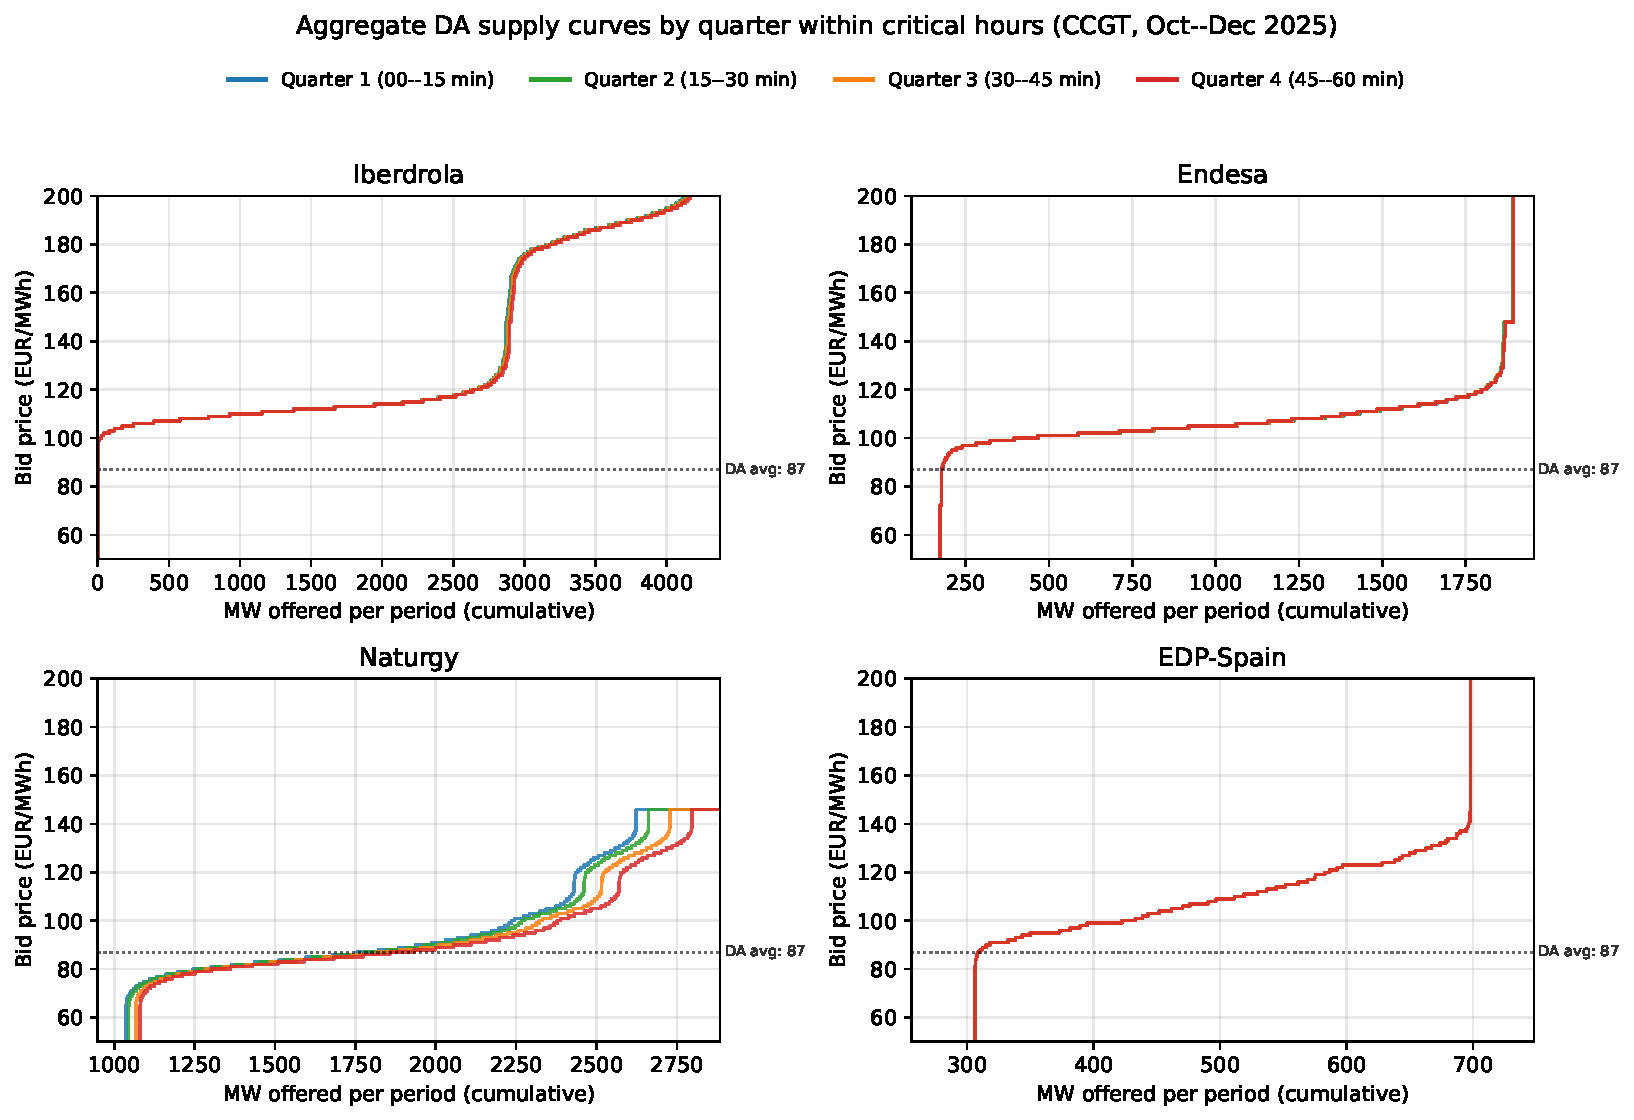
\includegraphics[width=\textwidth]{fig_per_firm_bid_curves_quarters_ccgt.pdf}
\caption{Critical hours (05:00--09:00, 16:00--23:00)}
\end{subfigure}\hfill
\begin{subfigure}[t]{0.49\textwidth}
\centering
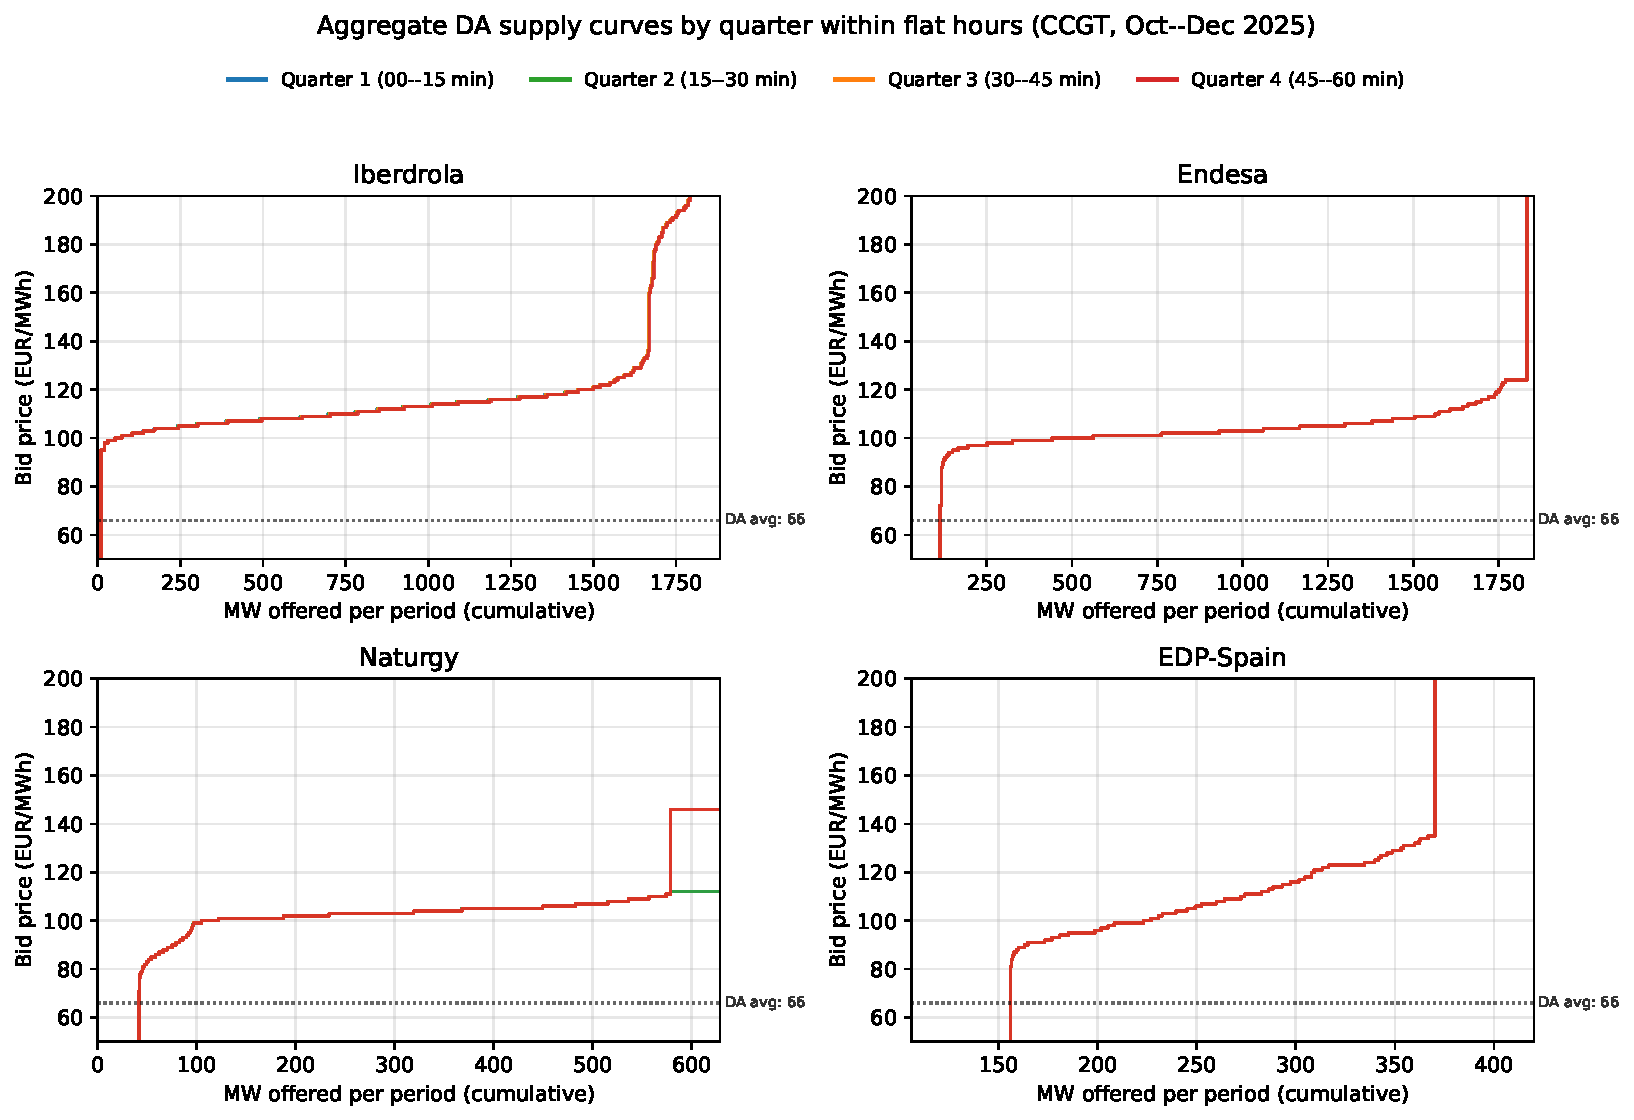
\includegraphics[width=\textwidth]{fig_per_firm_bid_curves_quarters_ccgt_flat.pdf}
\caption{Flat hours (01:00--04:00) --- falsification}
\end{subfigure}
\caption{Aggregate DA supply curves by quarter, CCGT, Oct--Dec 2025. Aggregated across $\sim$92 dates per (firm, hour, quarter) cell; day-specific quarter dispersion is smoothed in this visual.}
\end{figure}


% =====================================================================
\section{Per-firm CCGT bid curves and per-quarter pairs (IDA)}\label{sec:prov:ida_ccgt}
% =====================================================================

\textit{Reading} (\textbf{supportive}). IDA analogues of the main-text DA figures. In the post-MTU15-DA window the IDA pattern matches DA: dispersion concentrated in Naturgy and visible only in critical hours.

\begin{figure}[H]
\centering
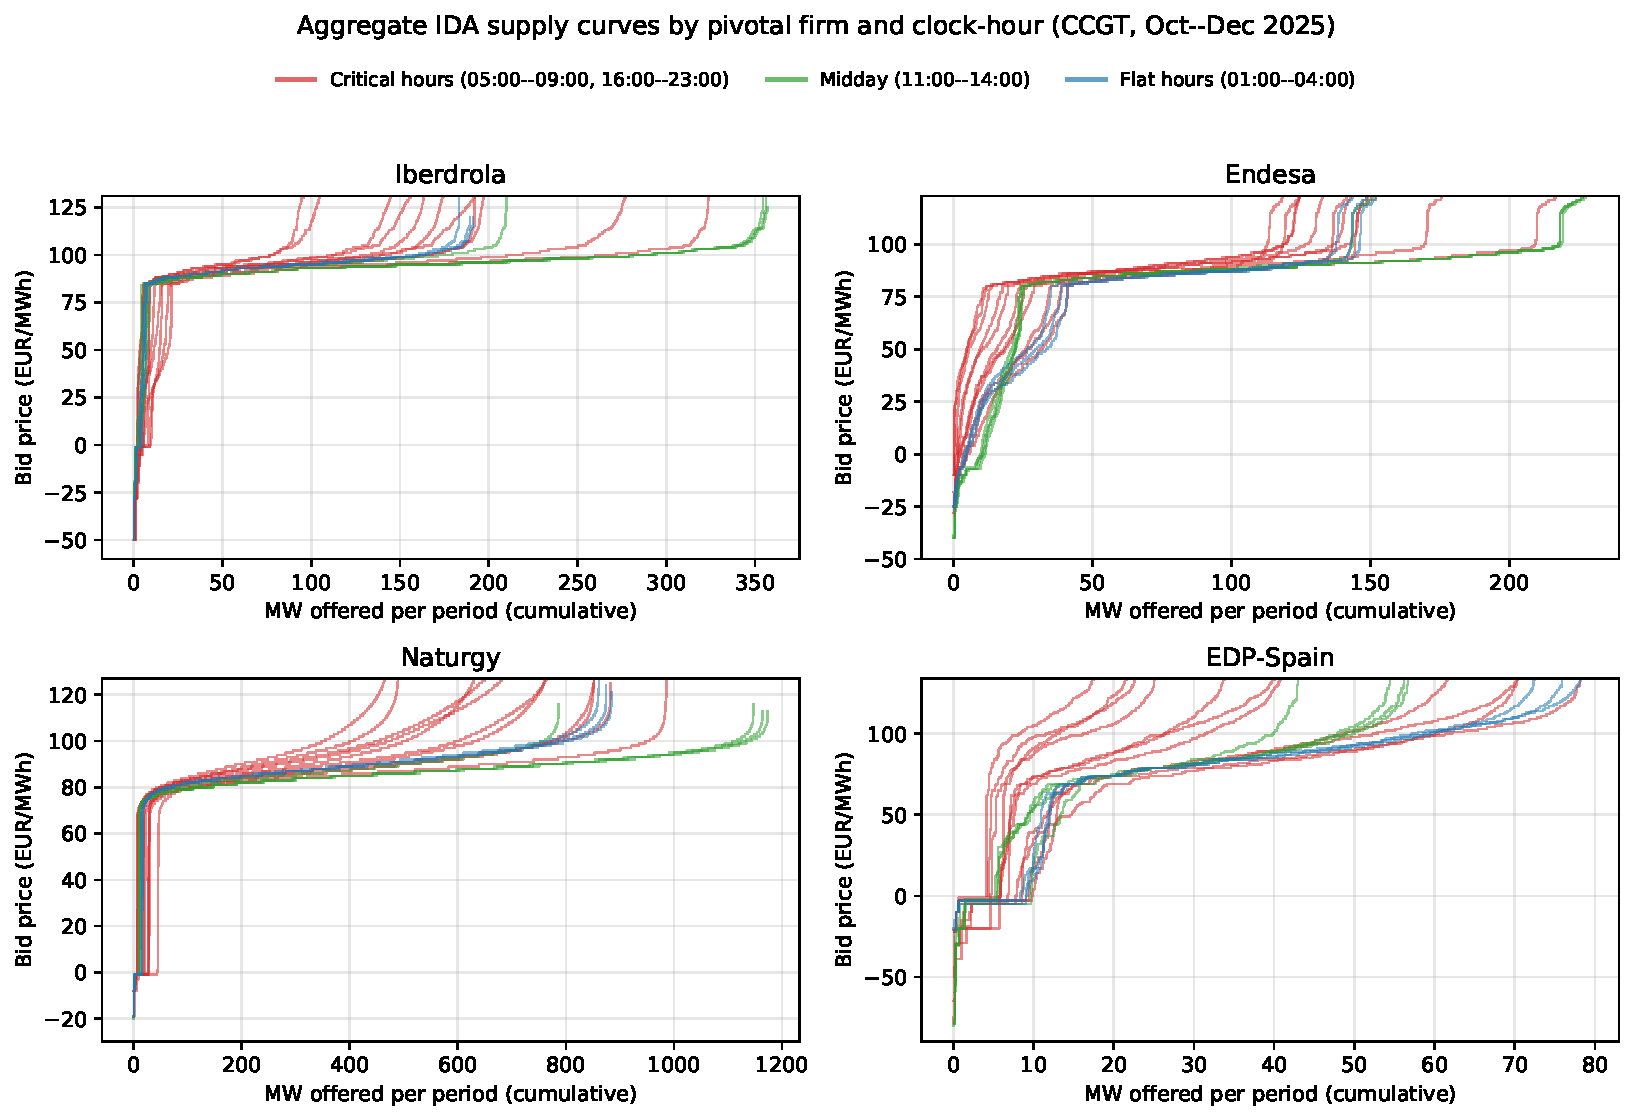
\includegraphics[width=0.95\textwidth]{fig_per_firm_bid_curves_ida.pdf}
\caption{Aggregate IDA supply curves by pivotal firm and clock-hour, CCGT, Oct--Dec 2025.}
\end{figure}

\begin{figure}[H]
\centering
\begin{subfigure}[t]{0.49\textwidth}
\centering
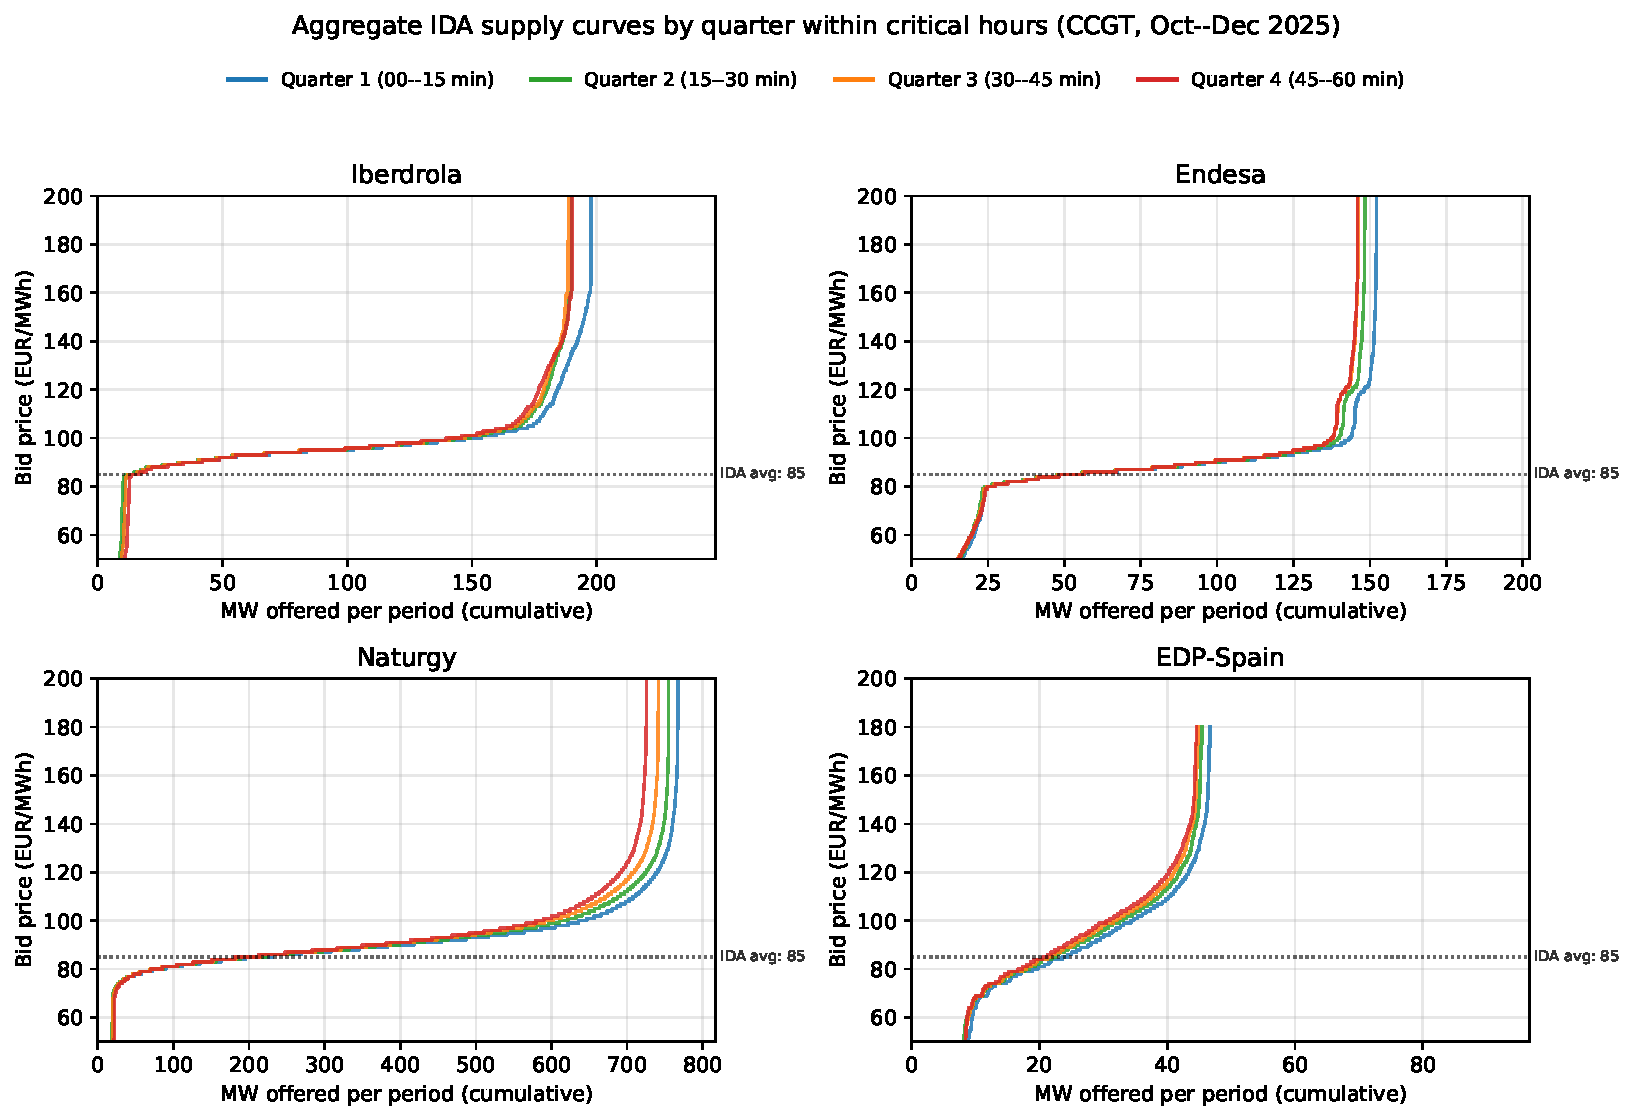
\includegraphics[width=\textwidth]{fig_per_firm_bid_curves_quarters_ccgt_ida.pdf}
\caption{Critical hours (05:00--09:00, 16:00--23:00)}
\end{subfigure}\hfill
\begin{subfigure}[t]{0.49\textwidth}
\centering
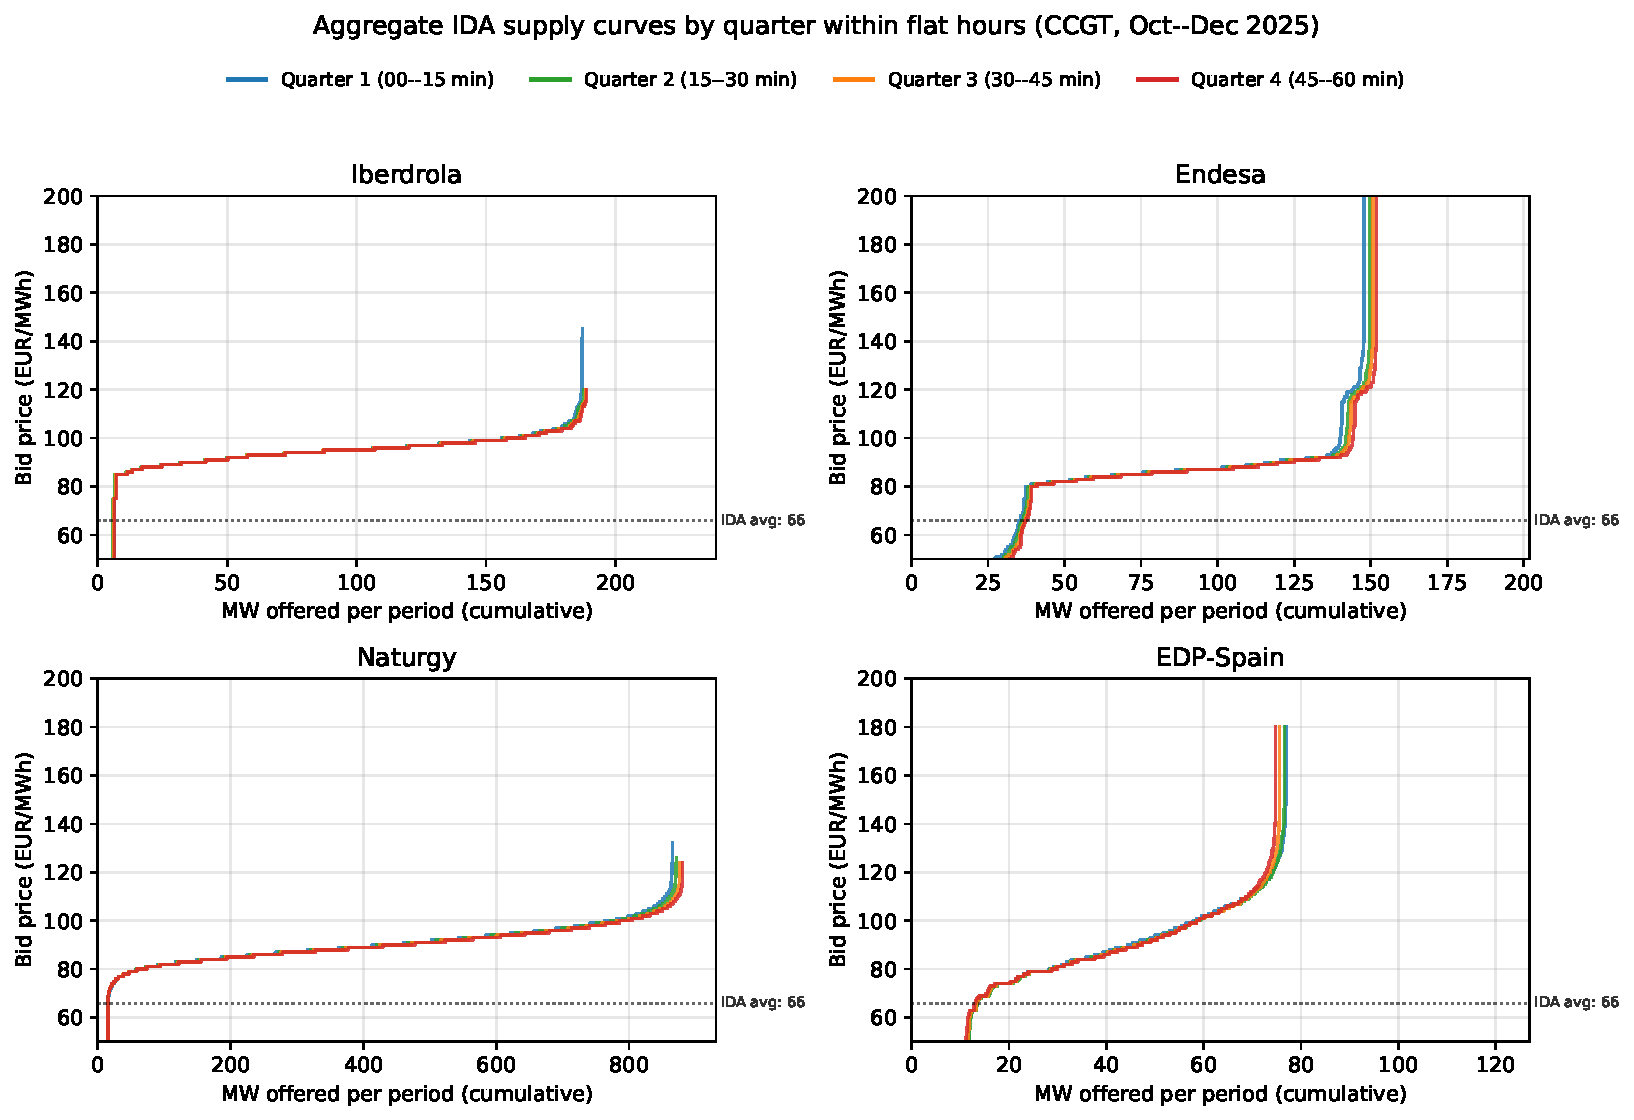
\includegraphics[width=\textwidth]{fig_per_firm_bid_curves_quarters_ccgt_ida_flat.pdf}
\caption{Flat hours (01:00--04:00)}
\end{subfigure}
\caption{Aggregate IDA supply curves by quarter, CCGT, Oct--Dec 2025.}
\end{figure}


% =====================================================================
\section{Per-quarter pump-storage demand curves (DA + IDA)}\label{sec:prov:pump_storage_quarters}
% =====================================================================

\textit{Reading} (\textbf{supportive}, as falsification). Pump-storage operators do not differentiate charge bids across the 4 quarters of a clock-hour --- the within-hour granularity is unused on this margin. Confirms pump-load as the clean mechanical falsifier.

\begin{figure}[H]
\centering
\begin{subfigure}[t]{0.49\textwidth}
\centering
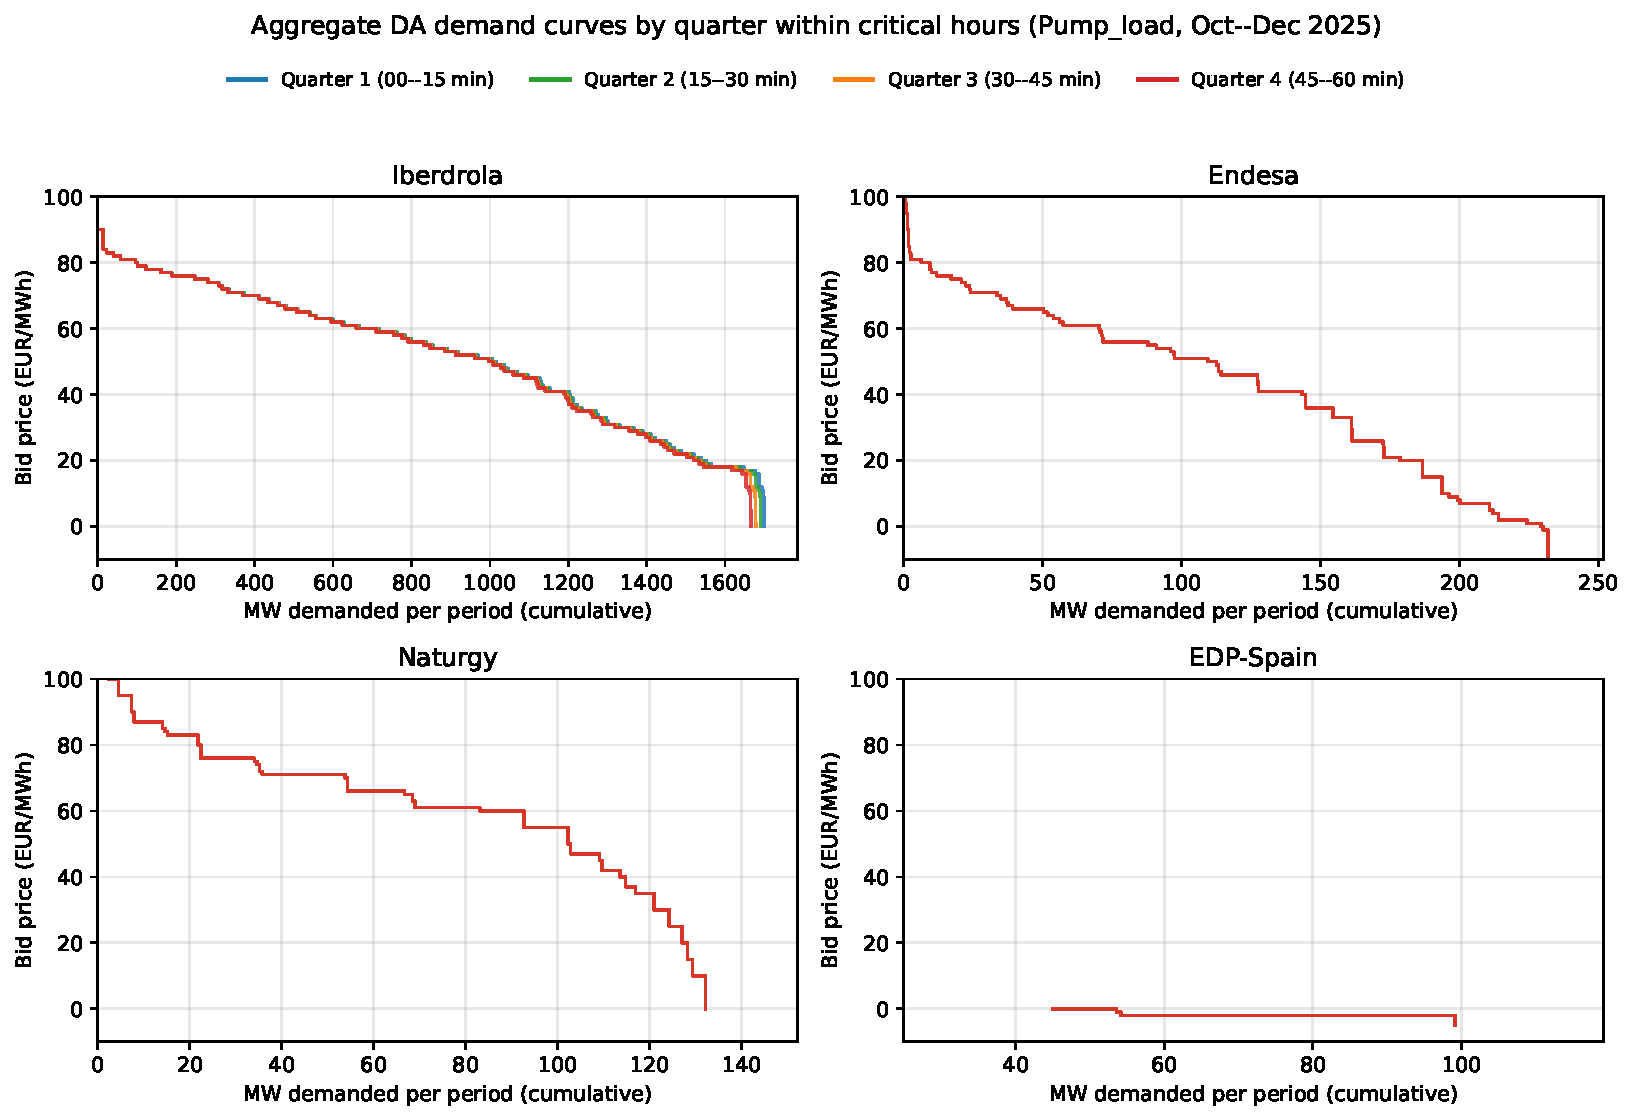
\includegraphics[width=\textwidth]{fig_per_firm_demand_curves_quarters_pump_load.pdf}
\caption{DA, critical hours}
\end{subfigure}\hfill
\begin{subfigure}[t]{0.49\textwidth}
\centering
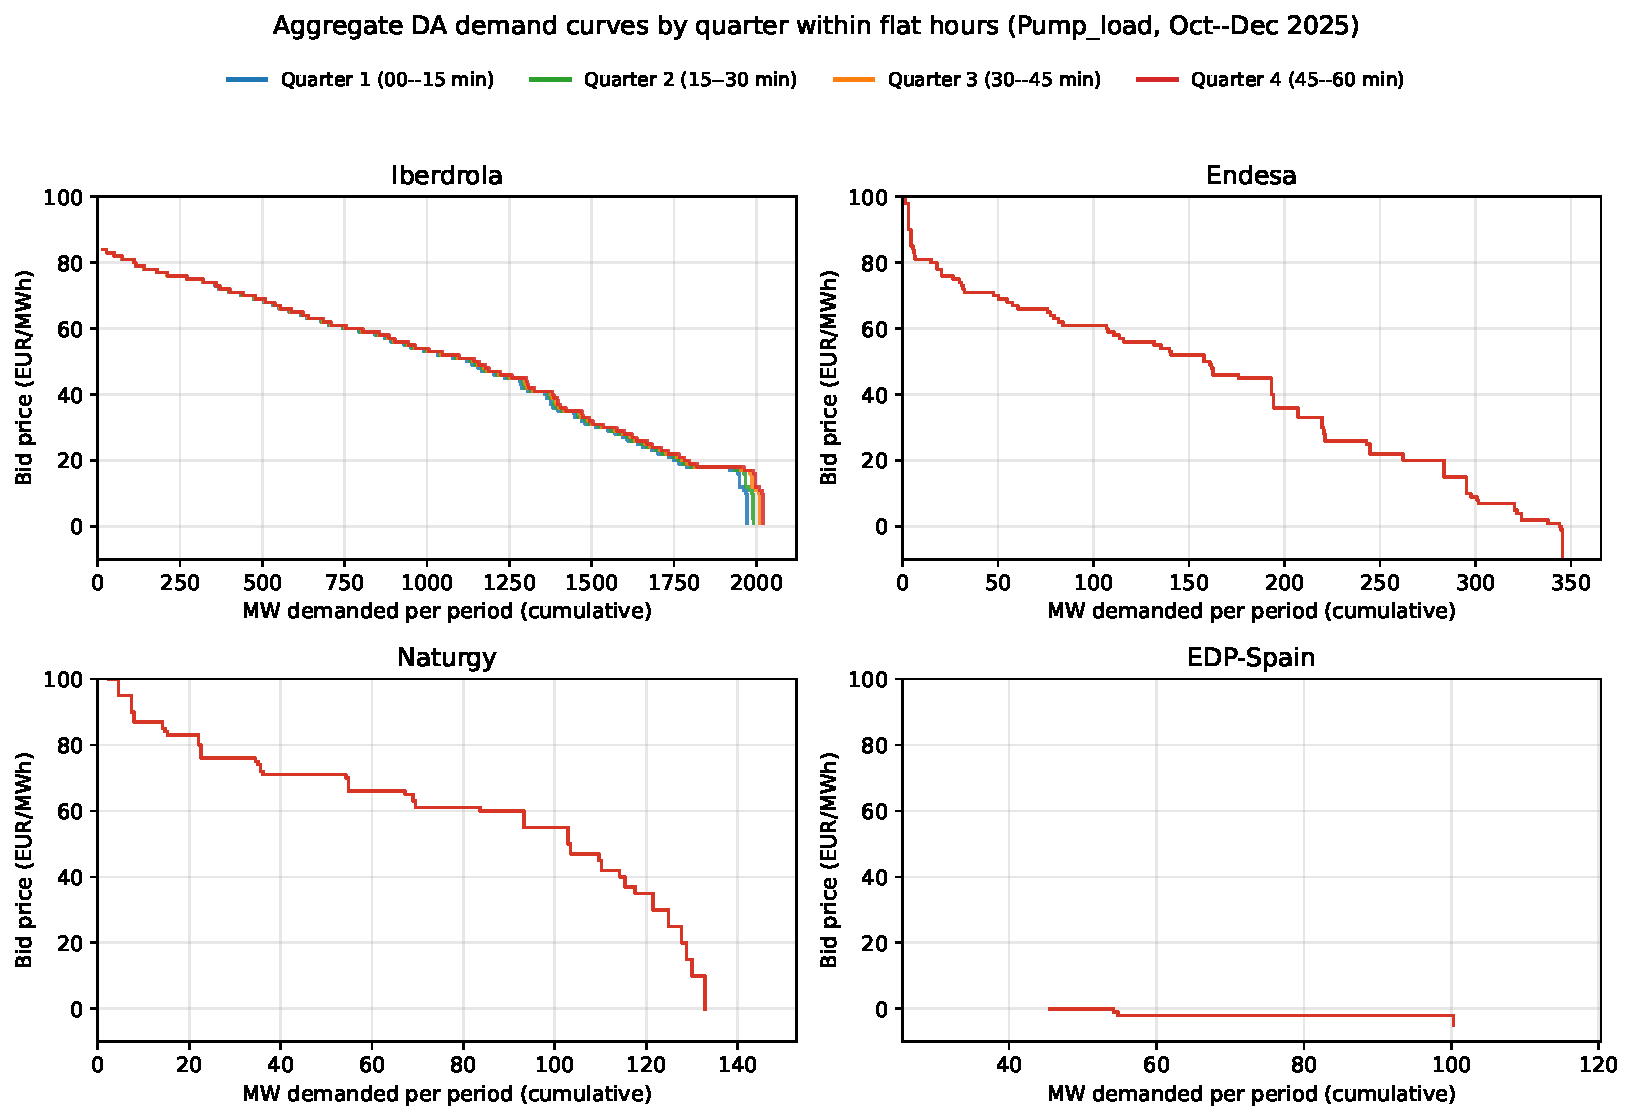
\includegraphics[width=\textwidth]{fig_per_firm_demand_curves_quarters_pump_load_flat.pdf}
\caption{DA, flat hours}
\end{subfigure}
\caption{Aggregate DA demand curves by quarter, pump-storage charge bids, Oct--Dec 2025.}
\end{figure}

\begin{figure}[H]
\centering
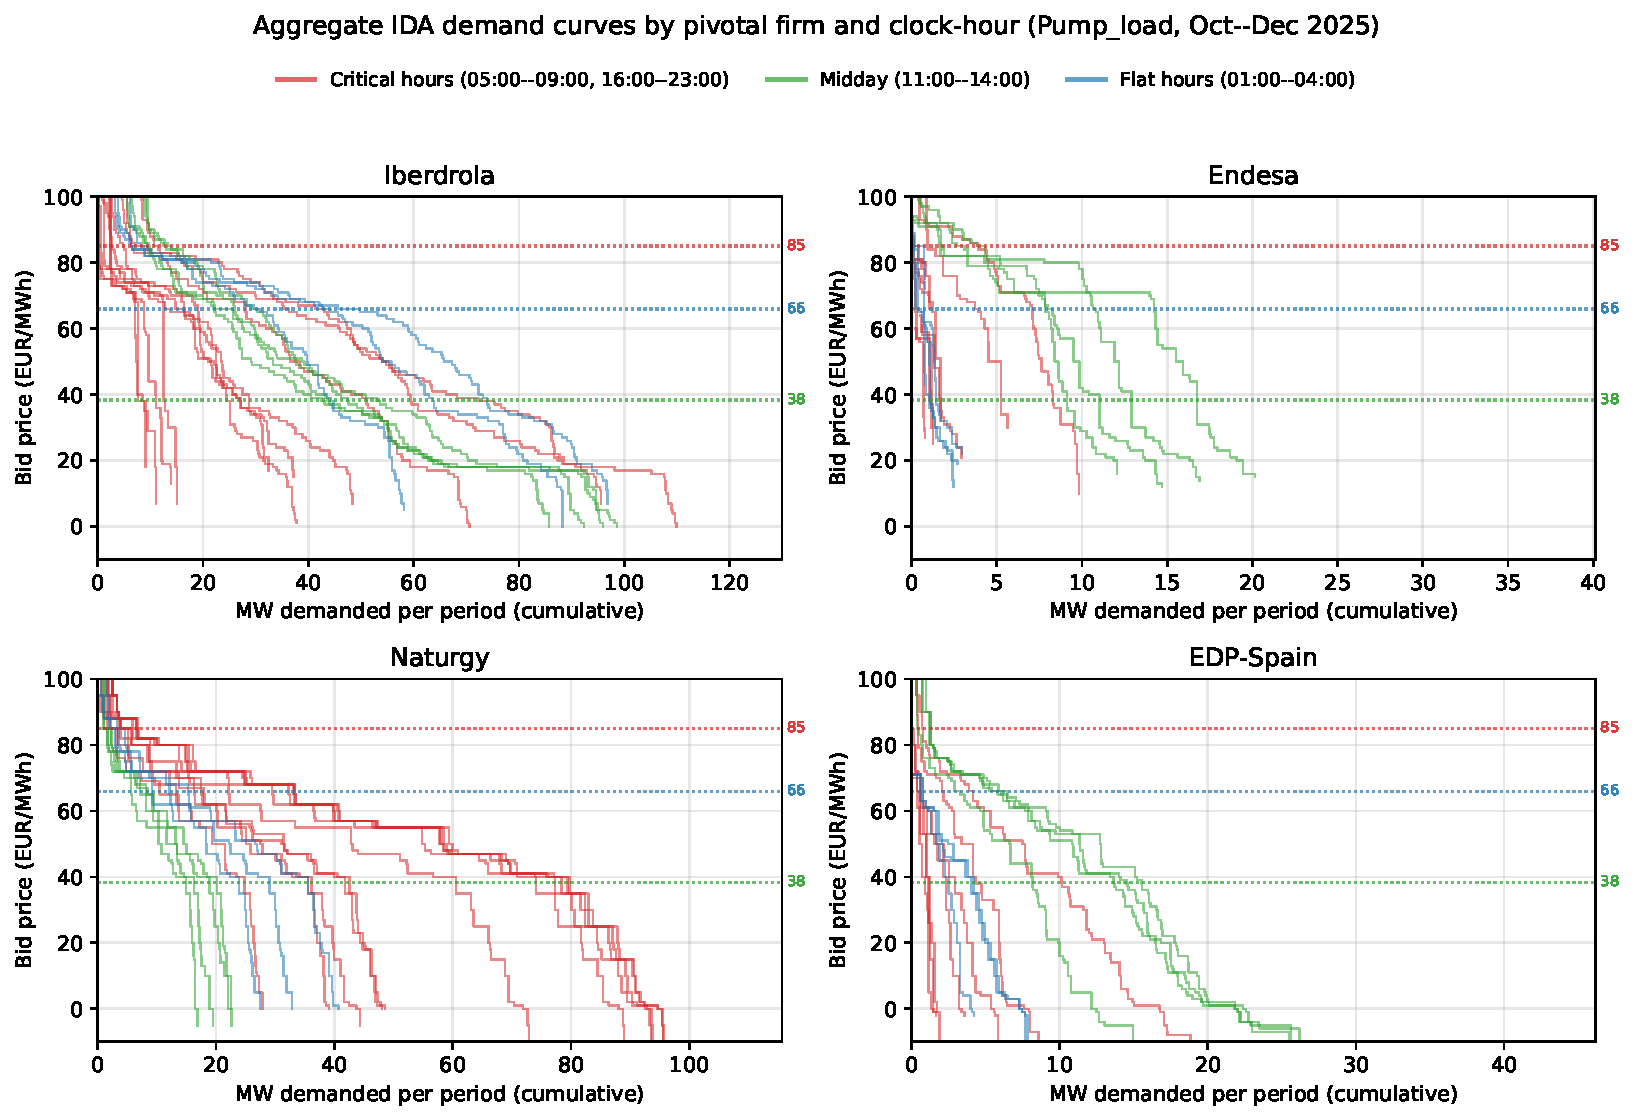
\includegraphics[width=0.95\textwidth]{fig_per_firm_demand_curves_pump_load_ida.pdf}
\caption{Aggregate IDA demand curves by pivotal firm and clock-hour, pump-storage charge bids, Oct--Dec 2025.}
\end{figure}

\begin{figure}[H]
\centering
\begin{subfigure}[t]{0.49\textwidth}
\centering
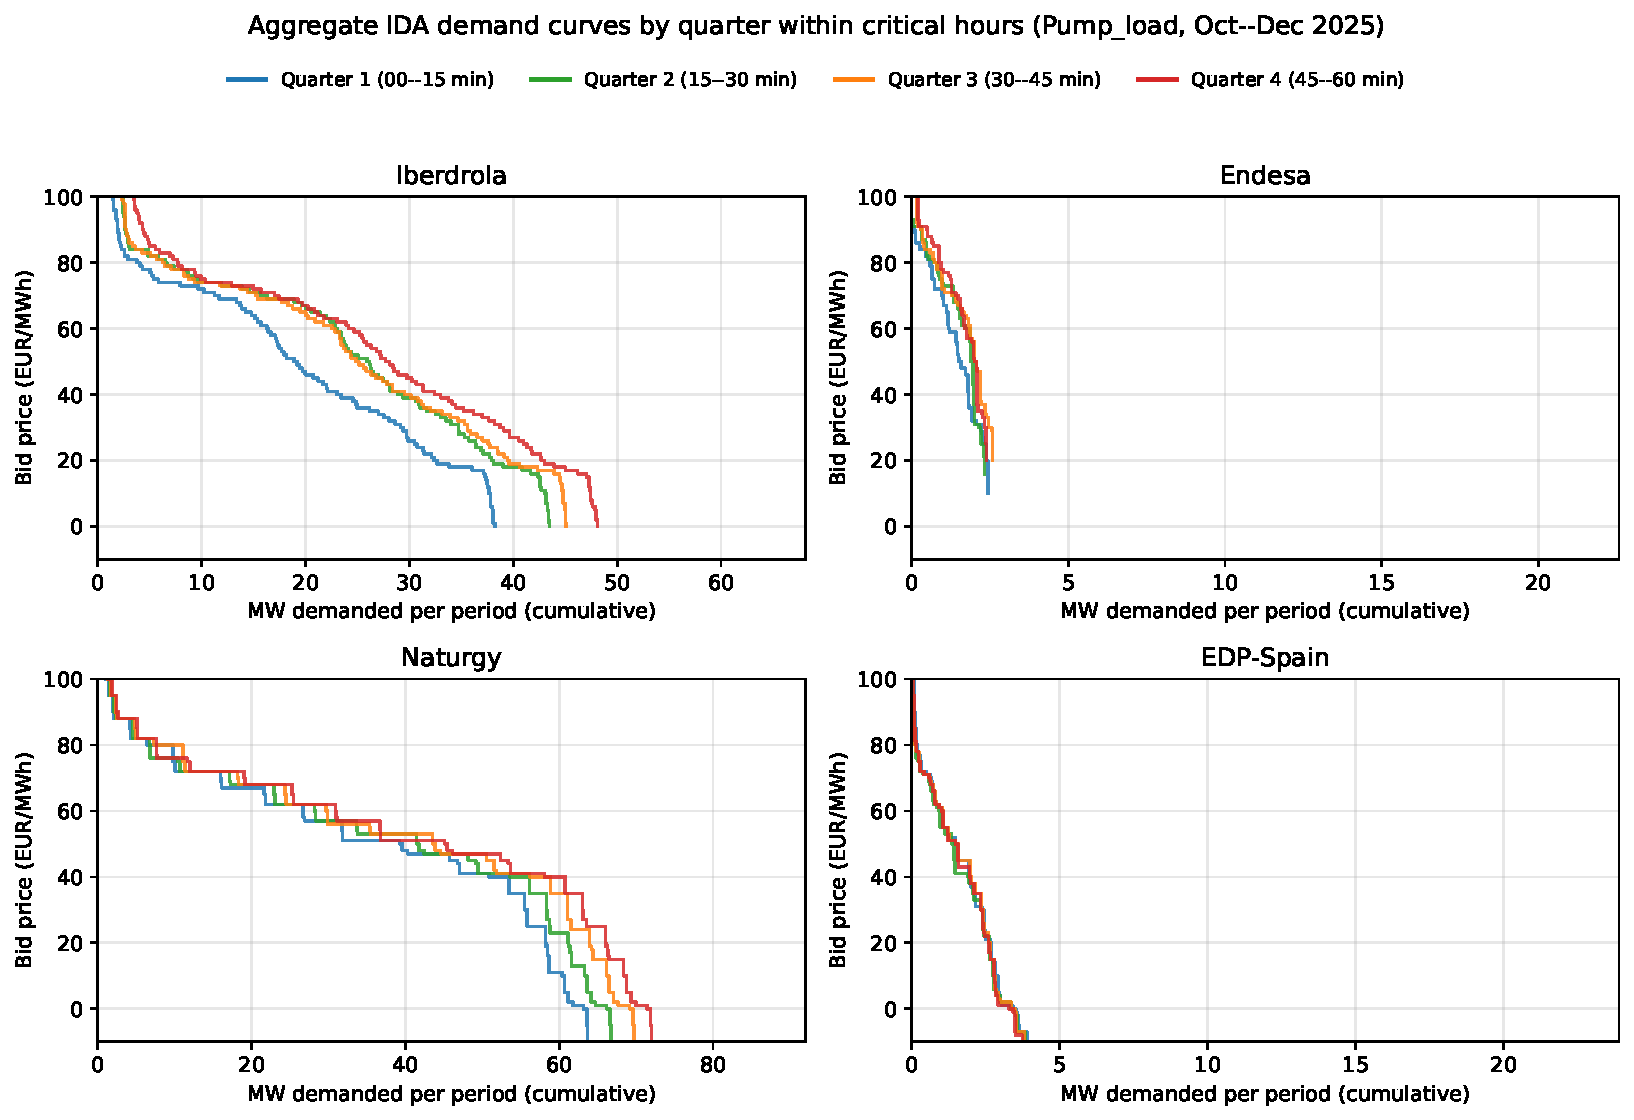
\includegraphics[width=\textwidth]{fig_per_firm_demand_curves_quarters_pump_load_ida.pdf}
\caption{IDA, critical hours}
\end{subfigure}\hfill
\begin{subfigure}[t]{0.49\textwidth}
\centering
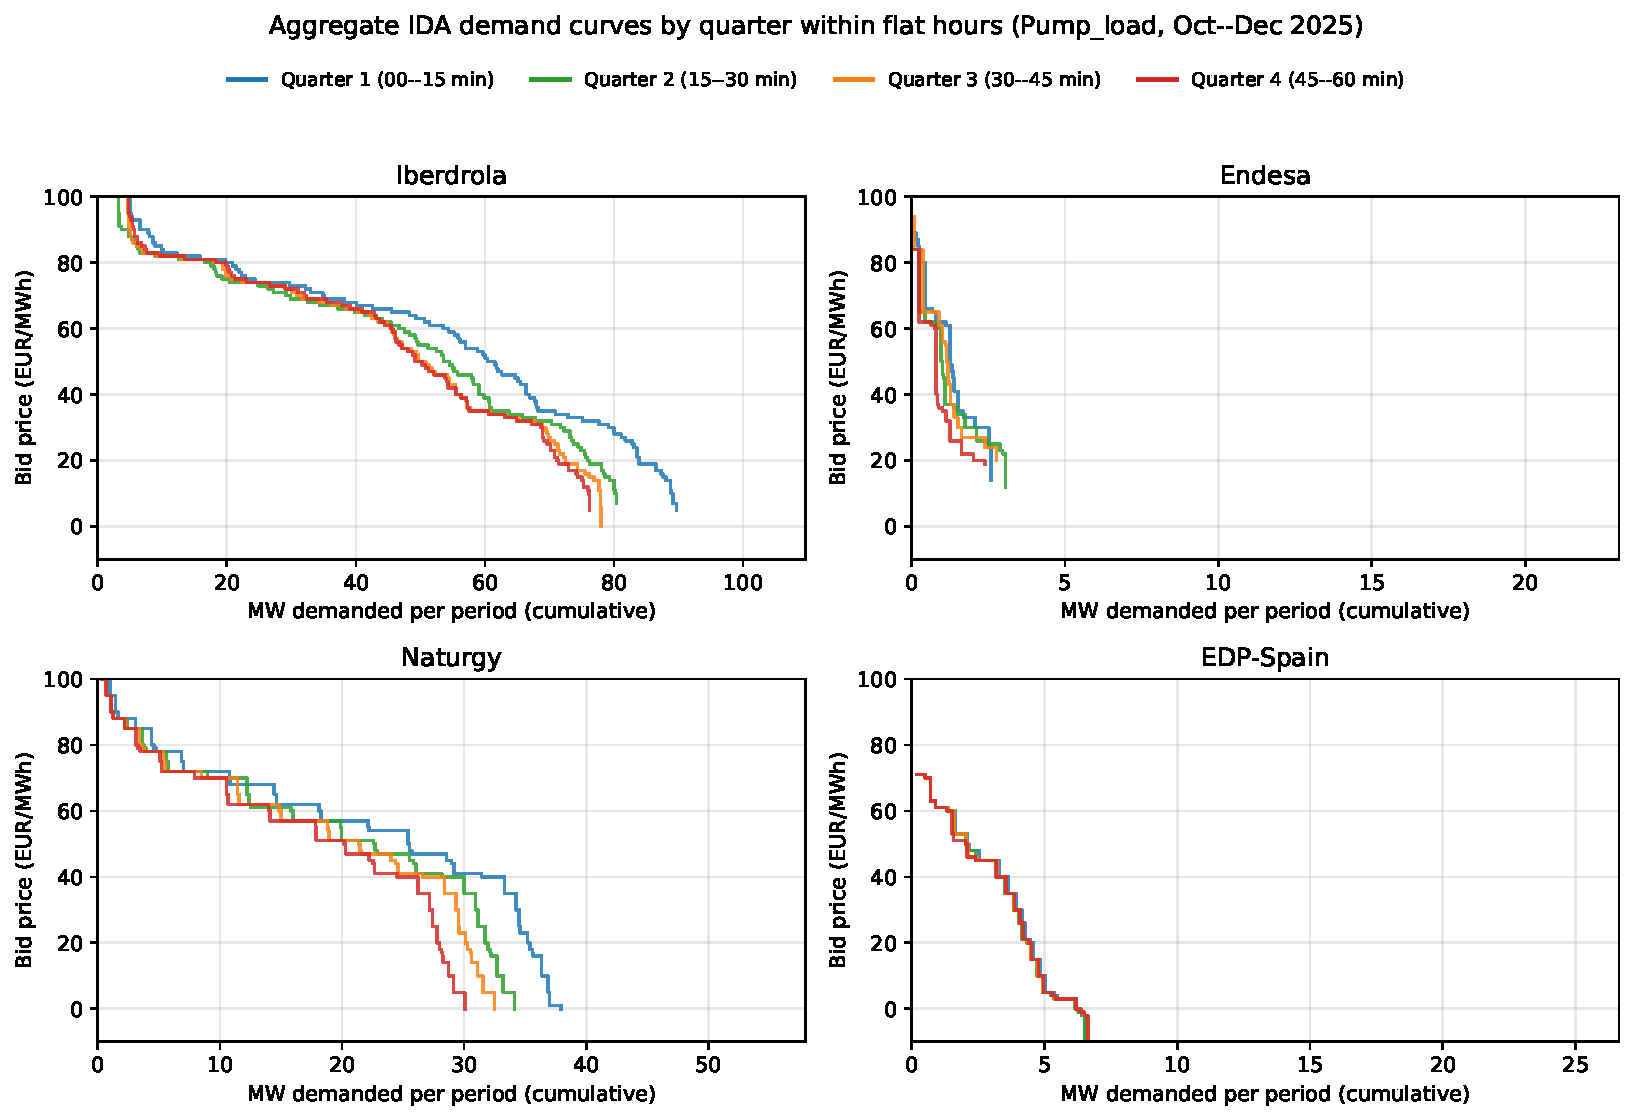
\includegraphics[width=\textwidth]{fig_per_firm_demand_curves_quarters_pump_load_ida_flat.pdf}
\caption{IDA, flat hours}
\end{subfigure}
\caption{Aggregate IDA demand curves by quarter, pump-storage charge bids, Oct--Dec 2025.}
\end{figure}


% =====================================================================
\section{Operational vs strategic decomposition (provisional)}\label{sec:prov:operational_strategic}
% =====================================================================

\textit{Reading} (\textbf{mixed}). The original main-paper Table reported a critical--flat asymmetry with the interpretation ``only Naturgy CCGT shows the strategic signature''. The IDA pre/post-blackout analysis above complicates this: under reforzada, all four firms show the strategic signature in IDA, not just Naturgy. The current main-paper framing is regime-specific to the DA Oct--Dec 2025 window. Until we have a unified read, the table is held here.

\begin{table}[H]
\centering
\caption{Original DA Oct--Dec 2025 critical--flat asymmetry table. Naturgy CCGT shows the strategic signature; renewables and retailer demand vary symmetrically across hour-classes (consistent with operational refinement); pump-storage is mechanical. Compare with the IDA pre/post-blackout finding in §\ref{sec:prov:ida_pre_post}.}
\label{tab:prov:operational_strategic_asym}
\begin{tabular}{l l l r r r}
\toprule
Channel & Tech & Firm & Critical & Flat & Crit $-$ Flat \\
\midrule
Strategic       & CCGT      & GN & 24.5 &  0.0 & $+24.5$ \\
Strategic       & CCGT      & IB &  5.8 &  3.9 & $+1.9$ \\
\addlinespace
Operational     & Wind      & IB & 97.2 & 97.3 & $-0.1$ \\
Operational     & Wind      & GN & 92.7 & 92.6 & $+0.1$ \\
Operational     & Wind      & HC & 93.7 & 93.8 & $-0.1$ \\
Operational     & Solar PV  & GN & 15.9 &  0.0 & $+15.9$ \\
Operational     & Retailer  & GE & 76.5 & 76.3 & $+0.2$ \\
Operational     & Retailer  & IB & 40.9 & 40.2 & $+0.7$ \\
Operational     & Direct\_consumer & IB & 96.0 & 95.3 & $+0.7$ \\
\addlinespace
Mechanical      & Pump\_load   & IB &  3.2 &  5.5 & $-2.3$ \\
Mechanical      & Pump\_load   & GE &  0.0 &  0.0 & $0.0$ \\
Mechanical      & Hydro\_pump  & IB &  0.4 &  0.0 & $+0.4$ \\
Mechanical      & Hydro\_pump  & GE &  0.0 &  0.0 & $0.0$ \\
\bottomrule
\end{tabular}
\end{table}


% =====================================================================
\section{REE post-clearing CCGT inclusion (Paths A, B, C)}\label{sec:prov:phf_minus_pdbf}
% =====================================================================

\textbf{Path A} (PHF $-$ PDBF, per unit) = IDA + REE post-IDA RT; \textbf{Path B} (\texttt{totalrp48preccierre} tipo 61$+$65, system) = REE PO 3.2 only; \textbf{Path C} (ENTSO-E A75 B04 actual $-$ PDBF, per firm) = full DA-to-metered.

\begin{figure}[H]
\centering
\includegraphics[width=0.97\textwidth]{../../figures/working/fig_ree_intervention_full.pdf}
\caption{\textbf{Full REE post-clearing intervention.} ESIOS archive 28 (\texttt{totalrp48preccierre}). Top: UP-redispatch GWh / month by channel; bottom: DOWN-redispatch (negative axis). RT-Tiempo Real (red, codes 61/65/66/69) is one of $\sim$8 channels; aFRR (capacity 23 + energy 80/81) is by volume the largest. mFRR (94/85), Gestión Desvíos (92), RR (96), RES curtailment (33/34) all add layers REE coordinates post-clearing.}
\end{figure}

\noindent Per-firm $\times$ per-technology Path A (PHF $-$ PDBF). Pre = 2024-01 $\to$ 2025-03; Post = 2025-05 $\to$ 2026-01.

\begin{table}[H]
\centering
\caption{PHF $-$ PDBF intervention by firm and technology, GWh / month.}
\label{tab:phf_pdbf_alltech}
\begin{tabular}{l l r r r r}
\toprule
Tech & Firm & Pre (GWh/mo) & Post (GWh/mo) & $\Delta$ (GWh/mo) & Ratio \\
\midrule
CCGT & GE & 213 & 413 & +200 & 1.94 \\
 & GN & 397 & 932 & +534 & 2.34 \\
 & HC & 42 & 94 & +52 & 2.25 \\
 & IB & 146 & 316 & +169 & 2.16 \\
\addlinespace
Hydro & GE & -58 & -253 & -195 & 4.33 \\
 & GN & 5 & -33 & -38 & -6.96 \\
 & HC & -0 & -11 & -11 & 40.05 \\
 & IB & 33 & -84 & -117 & -2.55 \\
\addlinespace
Hydro\_pump & GE & 2 & -15 & -17 & -7.14 \\
 & GN & 4 & 3 & -1 & 0.70 \\
 & IB & 23 & -1 & -24 & -0.03 \\
\addlinespace
Nuclear & GE & 241 & 23 & -218 & 0.10 \\
 & IB & 1 & -137 & -138 & -- \\
\addlinespace
Wind & GN & -9 & -36 & -27 & 4.02 \\
 & HC & -13 & -50 & -36 & 3.71 \\
 & IB & 8 & -81 & -89 & -10.63 \\
\addlinespace
Solar PV & GE & -0 & -0 & -0 & 9.13 \\
 & GN & -3 & -11 & -8 & 3.29 \\
 & HC & 0 & 1 & +1 & 6.26 \\
 & IB & 3 & -42 & -45 & -12.10 \\
\addlinespace
\bottomrule
\end{tabular}
\end{table}

\textit{Reading} (\textbf{supportive}). (i) CCGT $\times$2 for every firm; GN $+534$~GWh/mo (largest). (ii) Mirror decrease in Wind/Solar/Hydro/Nuclear: REE substitutes CCGT for clean tech post-PDBF. (iii) The full-intervention figure shows RT-Tiempo Real (red, our previous Path B) is one of $\sim$8 channels; aFRR energy and capacity reserves dominate the system-aggregate volume but are competitively priced. RT is the channel where pay-as-bid power matters.

\textit{Verdict} (\textbf{supportive}). Pay-as-bid pricing of RT-forced volume + zonal dominance (\S\ref{sec:prov:geo}) = local-monopoly channel. The full system picture (aFRR, mFRR, RR, RES curtailment) is shown for completeness; only RT involves pay-as-bid + local-grid binding.

\paragraph{Source data.}
\code{ree_intervention_full.py},
\code{ree_pdbf_to_phf_alltech.py}.


% =====================================================================
\section{Geographic CCGT concentration and RT2 pay-as-bid local power}\label{sec:prov:geo}
% =====================================================================

\noindent PO 3.2 redispatches relieve transmission-zone constraints, paid pay-as-bid. Zonal-dominant CCGT operator has local market power on RT bids. Zone assignment from plant city in \code{lista_unidades.csv}; capacity from ESIOS archive 110.

\begin{figure}[H]
\centering
\includegraphics[width=0.95\textwidth]{../../figures/working/fig_ccgt_zonal_capacity.pdf}
\caption{Spanish CCGT installed capacity (MW) by transmission zone and firm.}
\end{figure}

\begin{table}[H]
\centering
\caption{Per-zone CCGT capacity concentration. HHI on capacity shares ($\times 10\,000$).}
\label{tab:zonal_concentration}
\begin{tabular}{l r r r l r r}
\toprule
Zone & Plants & Capacity (MW) & \#~firms & Top firm & Top share (\%) & HHI \\
\midrule
Galicia  &  2 & 1\,247 & 2 & \textbf{GE}     & 68.6 & 5\,695 \\
Norte    & 10 & 2\,347 & 2$^\ast$ & non-Big-4$^\ast$ & 67.0 & 5\,577 \\
Aragón   &  3 & 1\,870 & 2$^\ast$ & non-Big-4$^\ast$ & 57.7 & 5\,119 \\
Centro   &  2 &   759 & 2 & \textbf{IB}     & 50.9 & 5\,001 \\
Levante  & 12 & 6\,117 & 3 & \textbf{GN}     & 40.6 & 3\,616 \\
Cataluña &  8 & 3\,788 & 4 & \textbf{GN}     & 44.5 & 3\,348 \\
Sur      & 13 & 5\,563 & 4 & \textbf{GN}     & 42.5 & 3\,040 \\
\bottomrule
\multicolumn{7}{l}{\footnotesize{$^\ast$~Norte and Aragón Big-4 share is small; top firms are non-Big-4 (Moeve, Engie, Total, Axpo).}} \\
\end{tabular}
\end{table}

\textit{Reading} (\textbf{supportive}). (i) Galicia (HHI 5\,695): 2 CCGTs only, GE 69\%. (ii) Centro (HHI 5\,001): 2 CCGTs, IB 51\% / GN 49\%. (iii) Cataluña/Levante/Sur (HHI 3\,000--3\,600): GN 40--45\% in each --- the three zones with heaviest reforzada. (iv) Norte/Aragón: Big-4 limited; non-Big-4 dominate.

\textit{Verdict} (\textbf{supportive}). GN's zonal dominance in the southern-mediterranean corridor pairs cleanly with the post-PDBF intervention story in \S\ref{sec:prov:phf_minus_pdbf}. Pay-as-bid RT2 + zonal dominance = local-monopoly channel that does not require flow-through to the auction. \emph{Caveats}: zone = plant city, not REE PO 3.2 books; capacity share is a static proxy; ESIOS archive 22 (\texttt{totalrpibcirest}, zonal IDA) would test it directly.

\paragraph{Source data.} \code{scripts/analysis/regulatory/ccgt_zonal_competition.py};
zone map at \code{data/external/ccgt_zonal_map.csv}.


% =====================================================================
\section{Are DA bid prices different on RT2-up days?}\label{sec:prov:bid_vs_rt2}
% =====================================================================

\noindent For each (CCGT unit, day), quantity-weighted DA sell-bid price, day labelled by RT2 magnitude $= \mathrm{PHF}_{\max} - \mathrm{PDBF}$: $\sim 0$ ($\le 100$ MWh), small\_up ($\le 1000$), large\_up ($> 1000$).

\begin{table}[H]
\centering
\caption{\textbf{DA, 2024-01 $\to$ 2026-01.} Quantity-weighted DA sell-bid price (EUR/MWh), median, by firm $\times$ regime $\times$ RT2-up state. Pre-blackout: 2024-01 $\to$ 2025-03. Post-blackout: 2025-05 $\to$ 2026-01.}
\label{tab:bid_vs_rt2}
\begin{tabular}{l l r r r r}
\toprule
Firm & Regime & $\sim 0$ RT2-up & small RT2-up & large RT2-up & Bid sensitivity \\
\midrule
GN & pre  & 843 & 850 & 851 & flat \\
GN & post & 844 & 834 & 841 & flat \\
\addlinespace
IB & pre  & 175 & 158 & 157 & flat \\
IB & post & 202 & 197 & 161 & --24 (large $-$ flat) \\
\addlinespace
GE & pre  & 1\,290 & 2\,168 & 2\,368 & +1\,078 (large $-$ flat) \\
GE & post & 2\,296 & 387   & 447   & --1\,849 (large $-$ flat) \\
\addlinespace
HC & pre  & 159 & 159 & 145 & flat \\
HC & post & 272 & 171 & 158 & --114 (large $-$ flat) \\
\bottomrule
\end{tabular}
\end{table}

\textit{Reading} (\textbf{mixed}). (i) GN median invariant at $\approx 840$ EUR/MWh across all six (regime, RT2-state) cells: cap-padded portfolio regardless of expected RT2 outcome. (ii) IB/HC near SRMC (150--200), mildly lower on large-RT2 days. (iii) GE volatile, dominated by sample composition.

\textit{Verdict} (\textbf{mixed}). GN does not need to clear DA; RT2 backstops at pay-as-bid. Caveat: conditional on \emph{ex-post} RT2 (not the cleanest test); the ex-ante ``REE-needs-me'' channel would need weather/load instruments. GE sample-composition noise blurs the read for one firm.

\paragraph{Source data.} \code{scripts/analysis/regulatory/ccgt_bid_vs_rt2_status.py};
\code{results/regressions/regulatory/ccgt_bid_vs_rt2/}.


% =====================================================================
\section{Decomposing $D_w$ into price and quantity components}\label{sec:prov:dw_decomp}
% =====================================================================

\paragraph{$D_w$, in full.}
Let cell $(f, u, d, h)$ index a firm $f$, unit $u$, date $d$, clock-hour $h$. The hour partitions into 4 quarters $q \in \{1,2,3,4\}$. In quarter $q$ the unit submits a multiset of price-quantity sell tranches with $p\in[\underline p, \overline p] \subset \mathbb{R}$ (Spanish SDAC: $\underline p = -500$, $\overline p = 4{,}000$ EUR/MWh; negative bids are admissible) and $x>0$ (MWh, energy for the quarter-slot). Let $c_{d,h}$ be the hour-mean clearing price and fix a strategic half-band of width $h = 50$ EUR/MWh around it. \textbf{We work throughout with band-restricted supply curves}: $N_q$ is the number of \emph{distinct} prices submitted in quarter $q$ \emph{within} $[c-h, c+h]$, and $x_{qk}$ is the sum of quantities at $p_{qk}$. The band-local quarter-$q$ supply curve is the right-continuous step function
\[
  S_q(p) \;=\; \sum_{k=1}^{N_q} x_{qk}\,\mathbf{1}\{p_{qk}\le p\}, \qquad p \in [c-h, c+h],
\]
with $S_q(c-h) = 0$ and $S_q(c+h) = M_q$ (the band-mass of quarter $q$). Infra-marginal mass below $c-h$ is excluded by construction: $D_w$ measures the within-band \emph{shape} of supply across quarters, not infra-marginal level offsets.

For two quarters $i, j$, the 1-D Wasserstein-1 distance is the $L^1$ area between cumulative curves, equivalently the $L^1$ distance between (extended) quantile functions:
\[
  W^{\text{band}}_1(S_i, S_j) \;=\; \int_{c-h}^{c+h}\!\big|S_i(p)-S_j(p)\big|\,dp \;=\; \int_{0}^{\max(M_i, M_j)}\!\big|S_i^{-1}(Q)-S_j^{-1}(Q)\big|\,dQ,
\]
where $S_q^{-1}(Q) = c+h$ for $Q > M_q$ pads the smaller curve to common total mass (Vallender, 1973). To isolate variation near the clearing price, weight by an (unnormalized) Epanechnikov-shape kernel:
\[
  K_h(p-c) \;=\; \max\!\left\{0,\;1 - \!\left(\frac{p-c}{h}\right)^{\!2}\right\}, \quad K_h \in [0,1], \quad K_h(c)=1,
\]
\[
  D^{(i,j)}_w \;=\; \int_{c-h}^{c+h}\! K_h(p-c)\,\big|S_i(p)-S_j(p)\big|\,dp \;\le\; W^{\text{band}}_1.
\]
$D_w$ has units EUR (quantity in MWh times price in EUR/MWh). The cell-level statistic is the max across the 6 pairs,
\[
  D^{\text{cell}}_w \;=\; \max_{1\le i<j\le 4}\,D^{(i,j)}_w.
\]
A cell is \emph{flagged} when $D^{\text{cell}}_w > 0$ (i.e.\ some within-hour bid variation falls inside the strategic band).

\paragraph{Decomposition.}
We split within-band variation into a price and a quantity channel:
\[
  \Delta q_{ij} \;=\; |M_i - M_j|\;\;[\text{MWh}],
  \qquad
  \Delta p_{ij} \;=\; \frac{1}{\min(M_i, M_j)}\int_{0}^{\min(M_i, M_j)}\!\!\big|S_i^{-1}(Q) - S_j^{-1}(Q)\big|\,dQ\;\;[\text{EUR/MWh}].
\]
$\Delta q$ captures band-mass mismatch (a quantity-only adjustment with prices on the common-mass portion held fixed). $\Delta p$ captures the mean price shift on the common-mass portion (a price-only adjustment with band-mass totals held fixed). Cell-level $\Delta p$, $\Delta q$ are the max over the 6 pairs.

\paragraph{Short proof of consistency.}
WLOG $M_i \le M_j$. Extending $S_i^{-1}(Q) = c+h$ for $Q \in (M_i, M_j]$ gives both quantile functions a common domain $[0, M_j]$ and common total mass $M_j$. The 1-D Wasserstein-1 duality for distributions with common mass (Vallender, 1973) gives
\[
  W^{\text{band}}_1 \;=\; \int_{c-h}^{c+h}\!\big|S_i(p) - S_j(p)\big|\,dp
  \;=\; \int_{0}^{M_j}\!\big|S_i^{-1}(Q) - S_j^{-1}(Q)\big|\,dQ.
\]
Split the right-hand integral at $Q = M_i$:
\begin{align*}
  W^{\text{band}}_1
    &= \underbrace{\int_0^{M_i}\!\big|S_i^{-1}(Q) - S_j^{-1}(Q)\big|\,dQ}_{=\;\Delta p_{ij}\,M_i\;\;\text{(definition of $\Delta p$)}}
    \;+\; \underbrace{\int_{M_i}^{M_j}\!\big(c{+}h - S_j^{-1}(Q)\big)\,dQ}_{=:\,R_{ij}}.
\end{align*}
The integrand of $R_{ij}$ lies in $[0, 2h]$ (since $S_j^{-1}(Q) \in [c-h, c+h]$), so $0 \le R_{ij} \le 2h\,\Delta q_{ij}$. Since $K_h \in [0,1]$ on the band,
\[
  D^{(i,j)}_w \;\le\; W^{\text{band}}_1 \;\le\; \Delta p_{ij}\,M_i + 2h\,\Delta q_{ij}.
\]

\emph{Limiting cases.} (i) If $M_i = M_j$, then $R_{ij}=0$ and $\Delta q_{ij}=0$, so $W^{\text{band}}_1 = \Delta p_{ij}\,M$: all variation is on the price channel. (ii) If $S_i^{-1} \equiv S_j^{-1}$ on $[0, M_i]$ (quantile functions coincide on common mass), then $\Delta p_{ij}=0$ and $W^{\text{band}}_1 = R_{ij} \in [0,\,2h\,\Delta q_{ij}]$: all variation is on the quantity channel. The two channels are orthogonal modes verifiable at the boundary cases. \hfill$\square$

\begin{table}[H]
\centering
\caption{\textbf{DA Oct--Dec 2025, CCGT.} $D_w$ decomposition into price- and quantity-channel components within $|p - c| \le 50$ EUR/MWh. Share-active = \% of cells with the component $> 0$; conditional median is over those active cells.}
\label{tab:dw_decomp}
\begin{tabular}{l l r r r r r}
\toprule
Firm & Hour & $n$ cells & $\Delta p$-active (\%) & $\Delta q$-active (\%) & med $\Delta p$ (EUR/MWh) & med $\Delta q$ (MWh) \\
\midrule
\textbf{GN} & critical & 14\,930 & \textbf{0.01} & \textbf{18.4} & 3.4 & 147 \\
GN & flat     &  4\,065 & 0.00 & 0.00 & --- & --- \\
\addlinespace
GE & critical &  5\,195 & 1.56 & 0.33 & 4.6 & 364 \\
GE & flat     &  1\,413 & 0.00 & 0.00 & --- & --- \\
\addlinespace
IB & critical &  7\,831 & 0.10 & 1.94 & 3.9 &  70 \\
IB & flat     &  2\,139 & 0.89 & 1.03 & 3.1 &  11 \\
\addlinespace
HC & critical &  2\,013 & 0.00 & 0.05 & --- &  60 \\
HC & flat     &    549 & 0.00 & 0.00 & --- & --- \\
\bottomrule
\end{tabular}
\end{table}

\textit{Reading} (\textbf{supportive}). (i) GN: 18.4\% $\Delta q$-active, 0.01\% $\Delta p$-active --- shaping is quantity-only. (ii) Flat hours: 0\% on both channels for GN/GE/HC. (iii) GE has the opposite mix (1.56\% $\Delta p$ vs 0.33\% $\Delta q$), both small. (iv) IB/HC: negligible.

\textit{Verdict} (\textbf{supportive}). GN fixes the price ladder near the cap and re-allocates quantity across the 4 quarters: the Cournot version of price-raising. Unit tests in \code{w1_decomposition.py} (identical $\to$ 0/0, same-price-diff-mass $\to$ 0/$+$, same-mass-diff-price $\to$ $+$/0) confirm the decomposition is mathematically correct.

\begin{figure}[H]
\centering
\includegraphics[width=0.98\textwidth]{../../figures/working/fig_dp_dq_hist_ccgt.pdf}
\caption{\textbf{Channel-level histograms of the decomposition, CCGT, DA Oct--Dec 2025.} Per-firm; left column $\Delta p$ (EUR/MWh), right column $\Delta q$ (MWh). Critical (red), midday (green), flat (blue). The y-axis is share of (firm $\times$ hour-class) cells; mass-at-zero in legend. Cleaner economic units than $D_w$: GN $\to$ $\Delta q$-only (right column busy, left empty); GE $\to$ $\Delta p$-leaning (left busy, right tight); IB/HC $\to$ near-empty.}
\end{figure}

\textit{Reading} (\textbf{supportive}). The channel histograms confirm Table~\ref{tab:dw_decomp} visually. GN's $\Delta q$ critical mass spans 0--300 MWh; GE's $\Delta p$ critical mass spans 0--25 EUR/MWh. Empirically $R_{ij} \ll 2h\,\Delta q_{ij}$ in our CCGT data (median $R / (2h\,\Delta q) = 0.003$): the extra band-mass sits near the top of the band, so the $\Delta q$ channel contributes little to $W_1^{\text{band}}$ even when $\Delta q$ is large. The decomposition into the two channels is mathematically exact in the limit cases but the upper bound $W_1 \le \Delta p\,M_i + 2h\,\Delta q$ is loose by $\sim$13$\times$ on average. Interpret $\Delta p$ and $\Delta q$ as channel indicators, not as additive contributions to $W_1$.

\paragraph{Source data.} \code{scripts/analysis/bid/w1_decomposition.py};
\code{scripts/analysis/bid/dp_dq_histograms.py}.

% =====================================================================
\section{Cournot reading + CNMC historical sanctions}\label{sec:prov:cournot_cnmc}
% =====================================================================

\textit{Reading} (\textbf{supportive}). Fixed price ladder near the cap + adjust only quantity = Cournot. Pure-economics equivalent to direct price-raising, but ``I never raised my offer price'' is a regulatorily defensible posture.

\begin{table}[H]
\centering
\caption{CNMC sanction resolutions in \code{docs/regulation/cnmc_resolutions/}.}
\label{tab:cnmc_sanctions}
\begin{tabular}{l l l l r}
\toprule
Year & Firm / Plant & Expediente & LSE article & Sanction \\
\midrule
2015 & Iberdrola hydro             & SNC-DE-046-14 & 64 muy grave (manipulation)   & 25.0 M EUR \\
2019 & \textbf{Naturgy CCGT$^\dagger$} & SNC-DE-175-17 & 65.34 grave (abnormal DA offers) & $\sim$7 M EUR \\
2019 & Endesa Besós 3              & SNC-DE-174-17 & 65.34 grave (abnormal DA offers) & 6.6 M EUR \\
2023 & Naturgy Sabón 3 (Galicia)   & ---           & 65.33 grave (RT abuse)        & confidential \\
2023 & Engie Castelnou             & SNC-DE-152-22 & grave (availability)          & --- \\
2023 & Ignis Escatrón 2            & SNC-DE-151-22 & grave (availability)          & --- \\
\bottomrule
\multicolumn{5}{l}{\footnotesize{$^\dagger$~Besós 4, PBCN 1/2, Sagunto 1/2/3, Málaga 1, SROQ 1 --- exactly our zonal map (\S\ref{sec:prov:geo}) Cataluña/Levante/Sur. CNMC-estimated minimum benefit 13.0 M EUR over 4 months.}} \\
\end{tabular}
\end{table}

\textit{Verdict} (\textbf{supportive}). 2019 GN sanction (SNC-DE-175-17) is the smoking-gun precedent: same plants, same zones, same mechanism (high DA $\to$ not despatched $\to$ systematically programmed at higher RT prices) over Oct 2016--Jan 2017. Our 2024--25 results show this practice continuing post-reforzada with the within-hour granularity reform as a new tool, and the DA bid posture invariant at 840 EUR/MWh. The 2023 Sabón 3 case extends the geography to Galicia (the GN/GE duopoly).

\paragraph{Separate channel.} \code{docs/regulation/cnmc_blackout_expedientes_2026.csv} = 56 expedientes opened 2026-04-16 for voltage-control violations (Art 65.8) tied to the blackout (IB 22, GE 17, GN 5). Distinct regulatory channel; not conflated with the auction-shaping practice.


% =====================================================================
\section{$D_w$ distributions across firms, technologies, and regimes}\label{sec:prov:dw_distributions}
% =====================================================================

\paragraph{DA — per firm $\times$ technology.}
\begin{figure}[H]
\centering
\includegraphics[width=0.98\textwidth]{../../figures/working/fig_dw_loghist_da.pdf}
\caption{\textbf{DA Oct--Dec 2025.} Per-(firm $\times$ tech) overlaid log-histograms of $D_w$, critical (red), midday (green), flat (blue), positive values only on $\log_{10}(D_w)$, bin width $= 0.1$ (factor $\approx 1.26$). Mass at $D_w = 0$ in the legend.}
\end{figure}

\paragraph{IDA — pre- vs post-blackout, side-by-side.}
\begin{figure}[H]
\centering
\includegraphics[width=0.98\textwidth]{../../figures/working/fig_dw_loghist_ida_merged.pdf}
\caption{\textbf{IDA $D_w$ histograms, pre- vs post-blackout merged.} Rows = firms; columns = (CCGT pre, CCGT post, Hydro pre, Hydro post). Per panel: critical (red), midday (green), flat (blue); mass-at-zero in the legend.}
\end{figure}

\begin{table}[H]
\centering
\caption{CCGT mass at $D_w = 0$ and conditional median $D_w$ ($D_w > 0$), by sample.}
\label{tab:dw_mass_median}
\begin{tabular}{l l r r r r}
\toprule
Sample & Firm & \% crit $= 0$ & \% flat $= 0$ & med($D_w \mid > 0$, crit) & med($D_w \mid > 0$, flat) \\
\midrule
\multirow{4}{*}{DA Oct--Dec 2025} & IB &  98 &  98 &   415 &   154 \\
                                  & GE &  98 & 100 & 1\,333 &  --- \\
                                  & GN &  77 & 100 & 5\,167 & 2\,287 \\
                                  & HC & 100 & 100 &  ---  &  --- \\
\midrule
\multirow{4}{*}{IDA pre-blackout} & IB &  90 &  93 &  142 &     6 \\
                                  & GE &  86 &  90 &  503 &   108 \\
                                  & GN &  70 &  91 &  504 &   242 \\
                                  & HC &  72 &  79 &  735 &   761 \\
\midrule
\multirow{4}{*}{IDA post-blackout}& IB &  80 &  94 &  229 &   342 \\
                                  & GE &  56 &  67 &  498 &   165 \\
                                  & GN &  46 &  62 &  836 &   322 \\
                                  & HC &  66 &  79 &  835 &   674 \\
\bottomrule
\end{tabular}
\end{table}

\textit{Reading} (\textbf{supportive}). (i) DA mass-at-zero $\approx$ identical critical vs flat for every firm except GN (77\% vs 100\%). (ii) IDA: post-blackout shifts mass-at-zero down for every firm; \%crit-at-0 $<$ \%flat-at-0 in every (firm, regime). (iii) Conditional median $D_w$ in critical hours $\approx$ 2--3$\times$ flat for GN, GE on IDA. (iv) Strategic signature (mass-asymmetry critical $<$ flat) appears only in CCGT and Solar~PV; operational categories overlap.

\paragraph{Source data.}
\code{scripts/analysis/bid/quarter_dissim_distributions.py}.


% =====================================================================
\section{The $q_1$ drop: CCGT-only DA disengagement}\label{sec:prov:q1_drop}
% =====================================================================

\noindent Pivotal-firm fleet DA-cleared volume ($q_1$) by technology. Same-calendar-month comparison isolates seasonality.

\begin{figure}[H]
\centering
\includegraphics[width=0.95\textwidth]{../../figures/working/fig_q_components_by_tech_weekly.pdf}
\caption{\textbf{Weekly three-component decomposition per technology}, Big-4 pivotal-firm aggregate. DA cleared (PDBC, blue) $+$ Bilaterals (PDBF $-$ PDBC, green) $+$ IDA $+$ REE-RT (PHF $-$ PDBF, red) = $q_{\text{final}}$ (PHF, black line). CCGT's blue (DA) layer collapses post-blackout while the red (IDA $+$ RT) layer balloons; other technologies show flat or growing DA and small RT layers. Vertical guides: MTU15-IDA (Mar 2025), Blackout (Apr 2025), MTU15-DA (Oct 2025).}
\end{figure}

\begin{figure}[H]
\centering
\includegraphics[width=0.95\textwidth]{../../figures/working/fig_q_components_ccgt_by_firm_weekly.pdf}
\caption{\textbf{Weekly three-component decomposition per CCGT firm.} Same construction. The DA $\to$ RT shift is firm-wide; the magnitude of the red (IDA $+$ RT) layer post-blackout is roughly proportional to the firm's zonal CCGT dominance (\S\ref{sec:prov:geo}): GN largest, IB / GE intermediate, HC smallest.}
\end{figure}

\begin{figure}[H]
\centering
\includegraphics[width=0.95\textwidth]{../../figures/working/fig_gap_dev_pdbf.pdf}
\caption{\textbf{Parallel-trends test on the post-clearing gap (PHF $-$ PDBF, IDA $+$ RT only).} Deviation from each tech's 2024 mean (zero baseline). Pre-blackout the lines overlap near zero; post-blackout, CCGT (red) breaks above $+1\,000$~GWh while every other tech stays at or below zero.}
\end{figure}

\begin{table}[H]
\centering
\caption{\textbf{Same-calendar-month DA-cleared volume by technology, GWh.} Pivotal-firm aggregate. Only CCGT collapses; every other technology grows or stays flat.}
\label{tab:q1_drop_by_tech}
\begin{tabular}{l r r r r r r r r r}
\toprule
 & \multicolumn{3}{c}{Dec 2024 $\to$ Dec 2025} & \multicolumn{3}{c}{Nov 2024 $\to$ Nov 2025} & \multicolumn{3}{c}{Aug 2024 $\to$ Aug 2025} \\
\cmidrule(lr){2-4}\cmidrule(lr){5-7}\cmidrule(lr){8-10}
Tech & Pre & Post & \% & Pre & Post & \% & Pre & Post & \% \\
\midrule
\textbf{CCGT} & \textbf{1444} & \textbf{244} & \textbf{-83\%} & \textbf{637} & \textbf{130} & \textbf{-80\%} & \textbf{532} & \textbf{360} & \textbf{-32\%} \\
Nuclear & 1253 & 2587 & +106\% & 933 & 1909 & +105\% & 1997 & 2243 & +12\% \\
Hydro & 1016 & 640 & -37\% & 509 & 611 & +20\% & 303 & 424 & +40\% \\
Hydro\_pump & 195 & 247 & +27\% & 182 & 341 & +87\% & 239 & 406 & +70\% \\
Wind & 732 & 696 & -5\% & 666 & 1081 & +62\% & 379 & 449 & +18\% \\
Solar PV & 57 & 34 & -40\% & 37 & 100 & +170\% & 37 & 136 & +268\% \\
\bottomrule
\end{tabular}
\end{table}

\textit{Reading} (\textbf{supportive}). (i) CCGT $q_1$ Big-4 fleet: Dec 2024 = 1\,444 GWh $\to$ Dec 2025 = 244 GWh (\textbf{$-83$\%}). Nov same comparison: $-80$\%. (ii) Nuclear, Wind, Hydro\_pump, Solar PV \emph{grow} in the same window. (iii) The intensive margin (per-cell mean MWh) is stable for CCGT at $\approx$300 MWh; what collapses is the extensive margin (number of unit-day-hours cleared at all). (iv) Renewables don't ``wait for RT2'' because REE doesn't call them up in PO 3.2 (their offers are constrained by primary energy availability); nuclear doesn't because it's baseload-must-clear. Only CCGT has the strategic option to stay out of DA.

\textit{Verdict} (\textbf{supportive}). The $q_1$ drop is mechanism-specific: CCGT firms with strong RT2 backstop (zonal dominance, \S\ref{sec:prov:geo}) increasingly bid above DA clearing under reforzada, get rescued by REE in RT2 at pay-as-bid (\S\ref{sec:prov:phf_minus_pdbf}), and post the 840 EUR/MWh cap-padded ladder we measure in \S\ref{sec:prov:bid_vs_rt2}--\S\ref{sec:prov:dw_decomp}. The $q_1$ collapse is the empirical face of the practice CNMC sanctioned in 2019 (\S\ref{sec:prov:cournot_cnmc}), now at fleet-wide scale.

\paragraph{Parallel-trends on the gap.}

\begin{table}[H]
\centering
\caption{IDA $+$ REE-RT gap by technology, mean GWh / month. Strips out bilaterals (PHF $-$ PDBF), so the residual is post-DA auction-cleared additions only.}
\label{tab:gap_pretrends}
\begin{tabular}{l r r r r}
\toprule
Tech & 2024 mean & 2025 pre-blackout & post-blackout & Post $-$ 2024 \\
\midrule
\textbf{CCGT}   & \textbf{848}  & \textbf{1\,069} & \textbf{1\,892} & \textbf{+1\,044} \\
Nuclear         &  279          &     207         &      85         &   $-$194  \\
Hydro           & $-$25         &  $-$202         &   $-$293        &   $-$268  \\
Hydro\_pump     &   29          &      24         &       4         &   $-$25   \\
Wind            & $-$11         &   $-$8          &   $-$63         &   $-$52   \\
Solar PV        &    1          &   $-$1          &   $-$40         &   $-$41   \\
\bottomrule
\end{tabular}
\end{table}

\textit{Reading on parallel-trends} (\textbf{supportive}). (i) Pre-blackout, all techs stay within $\pm$300 GWh of their 2024 baseline (see right panel of the parallel-trends figure). (ii) CCGT pre-drift +220 GWh from 2024 to 2025 pre-blackout, modest. (iii) Post-blackout, CCGT alone breaks parallel trends with $+1\,044$ GWh jump --- $\approx 5\times$ the pre-drift, a structural break not a continuation of trend. (iv) Nuclear/Hydro/Wind/Solar lose volume on the same channel ($-$25 to $-$268 GWh): REE displaces clean tech post-DA to make room for forced CCGT, consistent with the Path A all-tech table in \S\ref{sec:prov:phf_minus_pdbf}.

\paragraph{Identification implication.} The $q_2 / q_1$ Ito-Reguant denominator is itself endogenous to reforzada: the unit-day-hours that clear DA in 2025 are a selected sub-sample relative to 2024 (only the heaviest demand days where even the high bid clears). Same-calendar-month + unit FE help but don't fully address the composition shift. Cleaner approach: outcome on the \emph{bid} side (decision to stay out) rather than on the \emph{clearing} side (conditional $q_2 / q_1$).

\paragraph{Source data.} \code{scripts/analysis/firm/q1_drop_investigation.py};
outputs at \code{results/regressions/firm/q1_drop/}.


\end{document}
